% Capitolul 4: Ipoteza Pieței Eficiente (EMH)
% Statistica Piețelor Financiare
% Program de licență, Academia de Studii Economice din București

\documentclass[9pt, aspectratio=169, t]{beamer}

% Asigură încadrarea conținutului pe diapozitive
\setbeamersize{text margin left=8mm, text margin right=8mm}

%=============================================================================
% CONFIGURARE TEMĂ ȘI STIL
%=============================================================================
\usetheme{default}
% Utilizăm tema implicită pentru control curat al antetului/subsolului

% Paletă de Culori (potrivită cu PDF-ul Redispatch)
\definecolor{MainBlue}{RGB}{26, 58, 110}
\definecolor{AccentBlue}{RGB}{26, 58, 110}
\definecolor{IDAred}{RGB}{205, 0, 0}
\definecolor{DarkGray}{RGB}{51, 51, 51}
\definecolor{MediumGray}{RGB}{128, 128, 128}
\definecolor{LightGray}{RGB}{248, 248, 248}
\definecolor{VeryLightGray}{RGB}{235, 235, 235}
\definecolor{KeynoteGray}{RGB}{218, 218, 218}
\definecolor{SectionGray}{RGB}{120, 120, 120}
\definecolor{FooterGray}{RGB}{100, 100, 100}
\definecolor{Crimson}{RGB}{220, 53, 69}
\definecolor{Forest}{RGB}{46, 125, 50}
\definecolor{Amber}{RGB}{181, 133, 63}
\definecolor{Orange}{RGB}{230, 126, 34}
\definecolor{Purple}{RGB}{142, 68, 173}

% Fundal gradient (gradient Keynote exact 315°: alb la RGB 218,218,218)
\setbeamertemplate{background}{%
    \begin{tikzpicture}[remember picture, overlay]
        \shade[shading=axis, shading angle=315,
        top color=white, bottom color=KeynoteGray]
        (current page.south west) rectangle (current page.north east);
    \end{tikzpicture}%
}
% Culoare solidă de rezervă pentru compatibilitate
\setbeamercolor{background canvas}{bg=}

\setbeamercolor{palette primary}{bg=MainBlue, fg=white}
\setbeamercolor{palette secondary}{bg=MainBlue!85, fg=white}
\setbeamercolor{palette tertiary}{bg=MainBlue!70, fg=white}
\setbeamercolor{structure}{fg=MainBlue}
\setbeamercolor{title}{fg=IDAred}
\setbeamercolor{frametitle}{fg=IDAred, bg=}
\setbeamercolor{block title}{bg=MainBlue, fg=white}
\setbeamercolor{block body}{bg=VeryLightGray, fg=DarkGray}
\setbeamercolor{block title alerted}{bg=Crimson, fg=white}
\setbeamercolor{block body alerted}{bg=Crimson!8, fg=DarkGray}
\setbeamercolor{block title example}{bg=Forest, fg=white}
\setbeamercolor{block body example}{bg=Forest!8, fg=DarkGray}
\setbeamercolor{item}{fg=MainBlue}

% Culori subsol (suprascriu albastrul temei Madrid)
\setbeamercolor{author in head/foot}{fg=FooterGray, bg=}
\setbeamercolor{title in head/foot}{fg=FooterGray, bg=}
\setbeamercolor{date in head/foot}{fg=FooterGray, bg=}
\setbeamercolor{section in head/foot}{fg=FooterGray, bg=}
\setbeamercolor{subsection in head/foot}{fg=FooterGray, bg=}

% Stiluri marcatori (se aplică peste tot inclusiv în blocuri)
\setbeamertemplate{itemize item}{\color{MainBlue}$\boxdot$}
\setbeamertemplate{itemize subitem}{\color{MainBlue}$\blacktriangleright$}
\setbeamertemplate{itemize subsubitem}{\color{MainBlue}\tiny$\bullet$}
\setbeamertemplate{itemize/enumerate body begin}{\normalsize}
\setbeamertemplate{itemize/enumerate subbody begin}{\normalsize}

% Item spacing - compact style
\setlength{\leftmargini}{10pt}       % Level 1: minimal indent
\setlength{\leftmarginii}{10pt}      % Level 2: minimal additional indent
% Compact list spacing (zero extra space before/after lists in blocks)
\makeatletter
\def\@listi{\leftmargin\leftmargini \topsep 0pt \parsep 0pt \itemsep 0pt}
\def\@listii{\leftmargin\leftmarginii \topsep 0pt \parsep 0pt \itemsep 0pt}
\makeatother

\setbeamertemplate{navigation symbols}{}

%=============================================================================
% ANTET PERSONALIZAT
%=============================================================================
\setbeamertemplate{headline}{%
    \vskip10pt%
    \hbox to \paperwidth{%
        \hskip0.5cm%
        {\small\color{FooterGray}\thesection.\ \renewcommand{\hyperlink}[2]{##2}\insertsectionhead}%
        \hfill%
        \showlevel\hspace{4pt}%
        \textcolor{FooterGray}{\small\insertframenumber}%
        \hskip0.5cm%
    }%
    \vskip4pt%
    {\color{\currentlevelcolor}\hrule height 1.5pt}%
    \global\slidelevelnum=0%
    \gdef\currentlevelcolor{FooterGray}%
}

%=============================================================================
% SUBSOL PERSONALIZAT
%=============================================================================
\usepackage{fontawesome5}

\setbeamertemplate{footline}{%
    {\color{FooterGray}\hrule height 0.4pt}%
    \vskip4pt%
    \hbox to \paperwidth{%
        \hskip0.5cm%
        \textcolor{FooterGray}{\small Statistica Piețelor Financiare}%
        \hfill%
        \raisebox{-0.1em}{%
            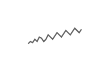
\begin{tikzpicture}[x=0.08em, y=0.08em, line width=0.4pt]
                \draw[FooterGray] (0,3) -- (1,4) -- (2,3.5) -- (3,5) -- (4,4) -- (5,6) -- (6,5.5) -- (7,4) -- (8,5) -- (9,7) -- (10,6) -- (11,5) -- (12,6.5) -- (13,8) -- (14,7) -- (15,6) -- (16,7.5) -- (17,9) -- (18,8) -- (19,7) -- (20,8.5) -- (21,10) -- (22,9) -- (23,8) -- (24,9.5);
            \end{tikzpicture}%
        }%
        \hskip0.5cm%
    }%
    \vskip6pt%
}

%=============================================================================
% PACHETE
%=============================================================================
\usepackage[utf8]{inputenc}
\usepackage[T1]{fontenc}
\usepackage{amsmath, amssymb, amsthm}
\usepackage{mathtools}
\usepackage{bm}
\usepackage{tikz}
\usetikzlibrary{arrows.meta, positioning, shapes, calc, decorations.pathreplacing, shadings}
\usepackage{booktabs}
\usepackage{multirow}
\usepackage{array}
\usepackage{graphicx}
\usepackage{hyperref}
\usepackage{colortbl}
\usepackage{pifont}
\usepackage{listings}
\lstset{language=Python, basicstyle=\ttfamily\scriptsize, keywordstyle=\color{MainBlue}\bfseries,
  commentstyle=\color{Forest}, stringstyle=\color{Crimson}, breaklines=true,
  frame=none, backgroundcolor=\color{VeryLightGray}, xleftmargin=2mm}
\hypersetup{colorlinks=true, linkcolor=MainBlue, urlcolor=MainBlue}
\graphicspath{{../../logos/}{../../charts/}{../../photos/}}
\hfuzz=7pt  % Suppress tiny overfull warnings (<7pt)
\vfuzz=4pt  % Suppress tiny vertical overfull warnings (<4pt)

%=============================================================================
% COMANDA QUANTLET
%=============================================================================
\newcommand{\quantlet}[2]{%
    \vspace{-0.25cm}%
    \hfill\href{#2}{%
        \raisebox{-0.15em}{
\includegraphics[height=0.7em]{ql_logo.png}}%
        \textcolor{MainBlue}{\tiny\ #1}%
    }\par%
}

%=============================================================================
% PAGINĂ TITLU PERSONALIZATĂ
%=============================================================================
\defbeamertemplate*{title page}{hybrid}[1][]
{
    \vspace{0.2cm}
    % Rând logo-uri - antet superior (cu linkuri clickabile)
    \begin{center}
        \href{https://www.ase.ro}{
\includegraphics[height=1.0cm]{ase_logo.png}}\hspace{0.3cm}%
        \href{https://theida.net}{
\includegraphics[height=1.0cm]{ida_logo.png}}\hspace{0.3cm}%
        \href{https://blockchain-research-center.com}{
\includegraphics[height=1.0cm]{brc_logo.png}}\hspace{0.3cm}%
        \href{https://www.ai4efin.ase.ro}{
\includegraphics[height=1.0cm]{ai4efin_logo.png}}\hspace{0.3cm}%
        \href{https://ipe.ro/new}{
\includegraphics[height=1.0cm]{acad_logo.png}}\hspace{0.3cm}%
        \href{https://www.digital-finance-msca.com}{
\includegraphics[height=1.0cm]{msca_logo.png}}%
    \end{center}

    \vspace{0.6cm}

    % Titlu principal cu logo-uri Q pe părți (cu linkuri clickabile)
    \begin{center}
        \begin{minipage}{0.1\textwidth}
            \centering
            \href{https://quantlet.com}{
\includegraphics[height=1.1cm]{ql_logo.png}}
        \end{minipage}%
        \begin{minipage}{0.78\textwidth}
            \centering
            {\LARGE\bfseries\usebeamercolor[fg]{title}\inserttitle}

            \vspace{0.3cm}

            {\usebeamerfont{subtitle}\usebeamercolor[fg]{title}\insertsubtitle}
        \end{minipage}%
        \begin{minipage}{0.1\textwidth}
            \centering
            \href{https://quantinar.com}{
\includegraphics[height=1.1cm]{qr_logo.png}}
        \end{minipage}
    \end{center}

    \vspace{0.6cm}

    % Autori (aliniere la stânga)
    \hspace{0.5cm}\begin{minipage}[t]{0.9\textwidth}
        \usebeamerfont{author}\insertauthor
    \end{minipage}

    \vspace{0.3cm}

    % Institut/Afilieri (aliniere la stânga)
    \hspace{0.5cm}\begin{minipage}[t]{0.9\textwidth}
        \raggedright\small\insertinstitute
    \end{minipage}
}

%=============================================================================
% MEDII PENTRU TEOREME
%=============================================================================
\theoremstyle{definition}
\setbeamertemplate{theorems}[numbered]
\newtheorem{defn}{Definiție}
\newtheorem{thm}{Teoremă}
\newtheorem{prop}{Propoziție}
\newtheorem{rmk}{Observație}

%=============================================================================
% CENTRED MINIPAGE
%=============================================================================
\newenvironment{cminipage}[1]{%
    \par\noindent\hfill\begin{minipage}{#1}\ignorespaces
}{%
    \end{minipage}\hfill\null\par
}

%=============================================================================
% COMENZI PERSONALIZATE
%=============================================================================
\newcommand{\E}{\mathbb{E}}
\newcommand{\Var}{\text{Var}}
\newcommand{\Cov}{\text{Cov}}
\newcommand{\Corr}{\text{Corr}}
\newcommand{\R}{\mathbb{R}}
\newcommand{\N}{\mathbb{N}}
\newcommand{\Z}{\mathbb{Z}}
\newcommand{\B}{\mathbf{B}}
\newcommand{\imark}{\textcolor{MainBlue}{\textbullet}}
\newcommand{\RMSE}{\text{RMSE}}
\newcommand{\MAE}{\text{MAE}}
\newcommand{\MAPE}{\text{MAPE}}

% Indicatoare nivel academic pe slide-uri  (numeric \ifnum — bulletproof in beamer templates)
\newcount\slidelevelnum
\global\slidelevelnum=0
\makeatletter
\newcommand{\slidelevel}[1]{%
    \global\slidelevelnum=0%
    \def\tmp@SL{#1}\def\tmp@SLy{Y3}\def\tmp@SLm{MSc}\def\tmp@SLp{PhD}%
    \ifx\tmp@SL\tmp@SLy \global\slidelevelnum=1\fi%
    \ifx\tmp@SL\tmp@SLm \global\slidelevelnum=2\fi%
    \ifx\tmp@SL\tmp@SLp \global\slidelevelnum=3\fi%
}
\makeatother
\gdef\currentlevelcolor{FooterGray}
\newcommand{\showlevel}{%
    \ifnum\slidelevelnum=1%
        \colorbox{Forest}{\strut\textcolor{white}{\sffamily\bfseries\fontsize{8}{9}\selectfont Y3}}%
        \gdef\currentlevelcolor{Forest}%
    \fi%
    \ifnum\slidelevelnum=2%
        \colorbox{MainBlue}{\strut\textcolor{white}{\sffamily\bfseries\fontsize{8}{9}\selectfont MSc}}%
        \gdef\currentlevelcolor{MainBlue}%
    \fi%
    \ifnum\slidelevelnum=3%
        \colorbox{Crimson}{\strut\textcolor{white}{\sffamily\bfseries\fontsize{8}{9}\selectfont PhD}}%
        \gdef\currentlevelcolor{Crimson}%
    \fi%
    \ifnum\slidelevelnum=0%
        \gdef\currentlevelcolor{FooterGray}%
    \fi%
}

%=============================================================================
% INFORMAȚII TITLU
%=============================================================================
\title[Statistica Piețelor Financiare]{Statistica Piețelor Financiare}
\subtitle{Capitolul 4: Ipoteza Pieței Eficiente (EMH)}
\author[D.T. Pele, A. Amza]{\texorpdfstring{\begin{tabular}[t]{@{}l@{}}Daniel Traian PELE \\ Antoaneta Amza\end{tabular}}{Daniel Traian PELE, Antoaneta Amza}}
\institute{Academia de Studii Economice din București\\
IDA Institute Digital Assets\\
Blockchain Research Center\\
AI4EFin Artificial Intelligence for Energy Finance\\
Academia Română, Institutul de Prognoză Economică\\
MSCA Digital Finance}
\date{}

\begin{document}

% Pagina de titlu (fără antet/subsol)
{
\setbeamertemplate{headline}{}
\setbeamertemplate{footline}{}
\begin{frame}
    \titlepage
\end{frame}
}

%=============================================================================
% OBIECTIVE DE ÎNVĂȚARE
%=============================================================================
\slidelevel{Y3}
\begin{frame}{Obiective de învățare}
\begin{cminipage}{0.95\textwidth}
\begin{block}{La finalul acestui capitol, veți fi capabili să:}
\begin{enumerate}
    \item[\textcolor{MainBlue}{\textbf{1.}}] \textbf{Definiți} eficiența informațională a pieței și cele trei forme (slabă, semi-tare, tare)
    \item[\textcolor{MainBlue}{\textbf{2.}}] \textbf{Formalizați} EMH utilizând modele martingal și mers aleator
    \item[\textcolor{MainBlue}{\textbf{3.}}] \textbf{Implementați} teste statistice pentru eficiența în formă slabă (weak-form) (autocorelație, runs, variance ratio)
    \item[\textcolor{MainBlue}{\textbf{4.}}] \textbf{Analizați} studii de eveniment pentru eficiența semi-tare
    \item[\textcolor{MainBlue}{\textbf{5.}}] \textbf{Evaluați} anomaliile de piață și provocările comportamentale la adresa EMH
    \item[\textcolor{MainBlue}{\textbf{6.}}] \textbf{Discutați} Ipoteza Pieței Adaptive ca sinteză modernă
\end{enumerate}
\end{block}
\end{cminipage}
\end{frame}

%=============================================================================
% CUPRINS
%=============================================================================
{
\setbeamertemplate{headline}{%
    \vskip10pt%
    \hbox to \paperwidth{\hskip0.5cm\hfill\hskip0.5cm}%
    \vskip4pt%
    {\color{FooterGray}\hrule height 0.4pt}%
}
\begin{frame}{}
    {\color{FooterGray}\hrule height 0.4pt}
    \vspace{0.1cm}
    {\Large\textcolor{IDAred}{\textbf{Cuprins}}}
    \vspace{0.2cm}
    {\small
    \begin{columns}[T]
        \begin{column}{0.48\textwidth}
            \begin{enumerate}
                \item Motivație
                \item Ipoteza Pieței Eficiente
                \item Cadrul matematic
                \item Eficiența în formă slabă (Weak-Form)
                \item Teste extinse de mers aleator
                \item Eficiența semi-tare (Semi-Strong)
            \end{enumerate}
        \end{column}
        \begin{column}{0.48\textwidth}
            \begin{enumerate}\setcounter{enumi}{6}
                \item Eficiența în formă tare (Strong-Form)
                \item Anomalii de piață
                \item Finanțe comportamentale
                \item Ipoteza Pieței Adaptive (AMH)
                \item Studii de caz și Exerciții
                \item Concluzii
            \end{enumerate}
        \end{column}
    \end{columns}
    }
\end{frame}
}

%#############################################################################
\section{Motivație}
%#############################################################################

\slidelevel{Y3}
\begin{frame}{Puteți bate piața?}
\begin{cminipage}{0.95\textwidth}
\begin{columns}[T]
\begin{column}{0.55\textwidth}
\begin{itemize}\setlength{\itemsep}{0pt}
    \item \textbf{Întrebarea centrală din finanțe:} poate un investitor să obțină constant randamente superioare indicelui de referință?
    \item Burton Malkiel (1973): ,,O maimuță legată la ochi, aruncând săgeți într-o pagină cu cotații bursiere, ar putea selecta un portofoliu la fel de bun ca cel ales cu grijă de experți.''
    \item \textbf{Fapt empiric:} peste 90\% din fondurile gestionate activ subperformează indicele de referință pe orizonturi de 15 ani (SPIVA Scorecard, 2024)
    \item Dacă prețurile reflectă deja toată informația disponibilă, nicio strategie nu poate genera sistematic \textbf{alpha}
\end{itemize}
\end{column}
\begin{column}{0.42\textwidth}
\begin{center}
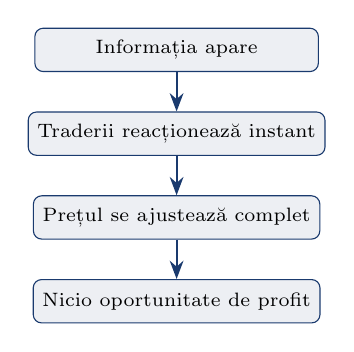
\begin{tikzpicture}[
    node distance=0.5cm,
    every node/.style={font=\scriptsize, align=center},
    phase/.style={draw=MainBlue, fill=MainBlue!8, rounded corners=3pt,
                  minimum width=3.6cm, minimum height=0.55cm}
]
\node[phase] (p1) {Informația apare};
\node[phase, below=of p1] (p2) {Traderii reacționează instant};
\node[phase, below=of p2] (p3) {Prețul se ajustează complet};
\node[phase, below=of p3] (p4) {Nicio oportunitate de profit};
\draw[-{Stealth}, MainBlue, thick] (p1) -- (p2);
\draw[-{Stealth}, MainBlue, thick] (p2) -- (p3);
\draw[-{Stealth}, MainBlue, thick] (p3) -- (p4);
\end{tikzpicture}
\end{center}
\end{column}
\end{columns}
\end{cminipage}
\end{frame}

\slidelevel{Y3}
\begin{frame}{Context istoric}
\begin{cminipage}{0.95\textwidth}
\renewcommand{\arraystretch}{1.2}
\begin{center}
\begin{tabular}{lll}
\toprule
\textbf{An} & \textbf{Autor} & \textbf{Contribuție} \\
\midrule
1900 & Louis Bachelier & Teză: prețurile acțiunilor urmează un mers aleator \\
1953 & Maurice Kendall & Prețurile acțiunilor britanice nu prezintă tipare \\
1965 & Eugene Fama & ,,Random Walks in Stock Market Prices'' \\
1965 & Paul Samuelson & ,,Proof That Properly Anticipated Prices Fluctuate Randomly'' \\
1970 & Eugene Fama & Taxonomia formală EMH: slabă, semi-tare, tare \\
1991 & Eugene Fama & EMH revizuită: predictibilitate, studii de eveniment \\
2004 & Andrew Lo & Ipoteza Pieței Adaptive (AMH) \\
2013 & Fama \& Shiller & Premiul Nobel (viziuni opuse despre eficiență) \\
\bottomrule
\end{tabular}
\end{center}
\end{cminipage}
\end{frame}

%#############################################################################
\section{Ipoteza Pieței Eficiente}
%#############################################################################

\slidelevel{Y3}
\begin{frame}{Definiția eficienței informaționale}
\begin{cminipage}{0.95\textwidth}
\begin{defn}[Piață eficientă --- Fama, 1970]
O piață este \textbf{eficientă informațional} dacă prețurile în orice moment $t$ reflectă pe deplin toată informația disponibilă $\Omega_t$. Formal: $P_t = \E[P_t \mid \Omega_t]$, unde $\Omega_t$ este mulțimea informațiilor disponibile la momentul $t$.
\end{defn}

\vspace{0.15cm}
\begin{itemize}\setlength{\itemsep}{0pt}
    \item \textbf{Implicație:} nicio strategie bazată pe $\Omega_t$ nu poate genera randamente așteptate peste randamentul de echilibru
    \item Modificările de preț răspund doar la \textbf{informații noi} (surprize), impredictibile prin definiție
    \item EMH este o \textbf{ipoteză compusă}: eficiență + un model de echilibru al randamentelor așteptate
\end{itemize}

\begin{alertblock}{Problema ipotezei compuse (Joint Hypothesis Problem)}
\begin{itemize}\setlength{\itemsep}{0pt}
    \item Nu putem testa eficiența izolat --- orice test necesită un model de evaluare a activelor (Capital Asset Pricing Model, CAPM; Arbitrage Pricing Theory, APT; etc.). O respingere poate însemna ineficiență \textit{sau} un model greșit.
\end{itemize}
\end{alertblock}
\end{cminipage}
\end{frame}

\slidelevel{Y3}
\begin{frame}{Cele trei forme ale EMH}
\begin{cminipage}{0.95\textwidth}
\begin{center}
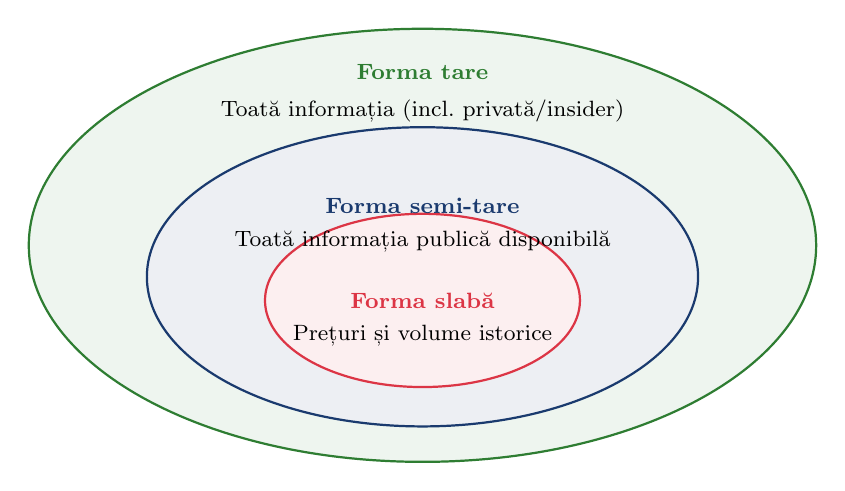
\begin{tikzpicture}[
    every node/.style={font=\small, align=center},
    circle1/.style={draw=Forest, fill=Forest!8, thick, ellipse, minimum width=10cm, minimum height=5.5cm},
    circle2/.style={draw=MainBlue, fill=MainBlue!8, thick, ellipse, minimum width=7cm, minimum height=3.8cm},
    circle3/.style={draw=Crimson, fill=Crimson!8, thick, ellipse, minimum width=4cm, minimum height=2.2cm}
]
\node[circle1] at (0,0) {};
\node[circle2] at (0,-0.4) {};
\node[circle3] at (0,-0.7) {};
\node[font=\footnotesize\bfseries, Forest] at (0, 2.2) {Forma tare};
\node[font=\footnotesize] at (0, 1.7) {Toată informația (incl.\ privată/insider)};
\node[font=\footnotesize\bfseries, MainBlue] at (0, 0.5) {Forma semi-tare};
\node[font=\footnotesize] at (0, 0.05) {Toată informația publică disponibilă};
\node[font=\footnotesize\bfseries, Crimson] at (0, -0.7) {Forma slabă};
\node[font=\footnotesize] at (0, -1.15) {Prețuri și volume istorice};
\end{tikzpicture}
\end{center}
\end{cminipage}
\end{frame}

\slidelevel{Y3}
\begin{frame}{Cele trei forme: rezumat}
\begin{cminipage}{0.95\textwidth}
\small
\renewcommand{\arraystretch}{1.2}
\begin{center}
\scriptsize
\begin{tabular}{llll}
\toprule
\textbf{Forma} & \textbf{Mulțimea info} & \textbf{Implicație} & \textbf{Ce exclude} \\
\midrule
\textbf{Slabă} & Prețuri, volume, rand.\ istorice & An.\ tehnică nu poate genera $\alpha$ & Medii mobile, tipare grafice \\
\textbf{Semi-tare} & Toată informația publică & An.\ fundamentală nu poate genera $\alpha$ & Filtre P/E, tranzacț.\ pe știri \\
\textbf{Tare} & Toată informația (incl.\ insider) & Niciun investitor nu are avantaj & Insider trading, info private \\
\bottomrule
\end{tabular}
\end{center}

\vspace{0.3cm}
\begin{itemize}\setlength{\itemsep}{0pt}
    \item Fiecare formă este \textbf{inclusă}: tare $\Rightarrow$ semi-tare $\Rightarrow$ slabă
    \item Dacă forma tare este valabilă, ambele forme mai slabe sunt automat valabile
    \item Majoritatea cercetărilor empirice se concentrează pe eficiența slabă și semi-tare
\end{itemize}
\end{cminipage}
\end{frame}

%#############################################################################
\section{Cadrul matematic}
%#############################################################################

\slidelevel{Y3}
\begin{frame}{Modelul jocului echitabil (Fair Game)}
\begin{cminipage}{0.95\textwidth}
\begin{defn}[Joc echitabil]
Fie $r_{t+1}$ randamentul unui activ. Piața este un \textbf{joc echitabil} în raport cu informația $\Omega_t$ dacă:
$\E[r_{t+1} - \E[r_{t+1} \mid \Omega_t] \mid \Omega_t] = 0$.
\end{defn}

\begin{itemize}\setlength{\itemsep}{0pt}
    \item Definim randamentul excesiv: $z_{t+1} = r_{t+1} - \E[r_{t+1} \mid \Omega_t]$
    \item Condiția de joc echitabil: $\E[z_{t+1} \mid \Omega_t] = 0$ --- erorile de prognoză sunt nedeplasate
    \item Nicio regulă de tranzacționare $\delta(\Omega_t)$ nu poate produce profit excesiv așteptat pozitiv: $\E[\delta(\Omega_t) \cdot z_{t+1}] = 0$
\end{itemize}

\begin{exampleblock}{Intuiție}
\begin{itemize}\setlength{\itemsep}{0pt}
    \item Un joc echitabil nu înseamnă că randamentele sunt zero --- înseamnă că randamentele \textbf{neașteptate} sunt zero în medie. Investitorii câștigă prima de risc, dar nu pot face sistematic mai bine.
\end{itemize}
\end{exampleblock}
\end{cminipage}
\end{frame}

\slidelevel{MSc}
\begin{frame}{Martingal și mers aleator}
\begin{cminipage}{0.95\textwidth}
\begin{columns}[T]
\begin{column}{0.48\textwidth}
\begin{block}{Martingal}
\begin{itemize}\setlength{\itemsep}{0pt}
    \item $\{P_t\}$ este martingal în raport cu $\Omega_t$ dacă:
    $$\E[P_{t+1} \mid \Omega_t] = P_t$$
    \item Prețurile nu au trend predictibil
    \item Mai slabă decât mersul aleator: permite varianță variabilă în timp
\end{itemize}
\end{block}
\end{column}
\begin{column}{0.48\textwidth}
\begin{block}{Mers aleator (Random Walk)}
\begin{itemize}\setlength{\itemsep}{0pt}
    \item \textbf{RW1:} $P_t = P_{t-1} + \varepsilon_t$, $\varepsilon_t \stackrel{iid}{\sim}(0, \sigma^2)$
    \item \textbf{RW2:} incremente independente dar nu identic distribuite
    \item \textbf{RW3:} incremente necorelate (cea mai slabă)
    \item RW1 $\Rightarrow$ RW2 $\Rightarrow$ RW3
\end{itemize}
\end{block}
\end{column}
\end{columns}

\vspace{0.3cm}
\begin{alertblock}{Distincție esențială}
\begin{itemize}\setlength{\itemsep}{0pt}
    \item EMH $\not\Leftrightarrow$ Mers aleator. EMH implică un \textbf{martingal} pentru prețurile ajustate la risc, nu neapărat incremente iid. Clusterizarea volatilității este compatibilă cu EMH.
\end{itemize}
\end{alertblock}
\end{cminipage}
\end{frame}

\slidelevel{MSc}
\begin{frame}{Cele trei tipuri de mers aleator: detalii}
\begin{cminipage}{0.95\textwidth}
\begin{defn}[RW1 --- Mers aleator cu incremente iid]
$P_t = \mu + P_{t-1} + \varepsilon_t$, unde $\varepsilon_t \stackrel{iid}{\sim}(0, \sigma^2)$. Incrementele sunt independente și identic distribuite. Cel mai restrictiv model.
\end{defn}

\vspace{0.15cm}
\begin{columns}[T]
\begin{column}{0.48\textwidth}
\begin{block}{RW2 --- Incremente independente}
\begin{itemize}\setlength{\itemsep}{0pt}
    \item $P_t = \mu + P_{t-1} + \varepsilon_t$
    \item $\varepsilon_t$ sunt independente dar \textbf{nu} identic distribuite
    \item Permite heteroscedasticitate necondiționată (de ex.\ volatilitatea se modifică între subperioade)
    \item Testabil prin: variance ratio, BDS test
\end{itemize}
\end{block}
\end{column}
\begin{column}{0.48\textwidth}
\begin{block}{RW3 --- Incremente necorelate}
\begin{itemize}\setlength{\itemsep}{0pt}
    \item $\Cov(\varepsilon_t, \varepsilon_s) = 0$ pentru $t \neq s$
    \item Dar pot exista dependențe neliniare: $\Cov(\varepsilon_t^2, \varepsilon_s^2) \neq 0$
    \item Compatibil cu modele GARCH
    \item Cel mai slab model --- autocorelațiile randamentelor sunt zero, dar cele ale randamentelor pătratice nu
\end{itemize}
\end{block}
\end{column}
\end{columns}
\end{cminipage}
\end{frame}

\slidelevel{MSc}
\begin{frame}[shrink=5]{Mersul aleator logaritmic (Logarithmic Random Walk)}
\begin{cminipage}{0.95\textwidth}
\begin{block}{Modelul}
\begin{itemize}\setlength{\itemsep}{0pt}
    \item Prețurile financiare urmează un \textbf{mers aleator geometric}:
    $$P_t = P_{t-1} \cdot e^{\mu + \sigma\varepsilon_t}, \quad \varepsilon_t \sim \mathcal{N}(0,1)$$
    \item Echivalent, log-prețurile urmează un mers aleator aritmetic:
    $$\ln P_t = \ln P_{t-1} + \mu + \sigma\varepsilon_t$$
    \item Log-randamentele sunt i.i.d.:
    $$r_t = \ln\frac{P_t}{P_{t-1}} = \mu + \sigma\varepsilon_t \stackrel{iid}{\sim} \mathcal{N}(\mu, \sigma^2)$$
\end{itemize}
\end{block}

\begin{columns}[T]
\begin{column}{0.48\textwidth}
\begin{itemize}\setlength{\itemsep}{0pt}
    \item \textbf{De ce logaritmic?}
    \item Prețurile nu pot fi negative: $P_t > 0$ întotdeauna
    \item Log-randamentele sunt aditiv compuse
    \item Consistent cu capitalizarea continuă
    \item Log-normalitatea implică cozi mai groase decât normalul simplu
\end{itemize}
\end{column}
\begin{column}{0.48\textwidth}
\begin{itemize}\setlength{\itemsep}{0pt}
    \item \textbf{Proprietăți:}
    \item $\E[\ln P_t] = \ln P_0 + \mu t$
    \item $\Var(\ln P_t) = \sigma^2 t$ (crește liniar)
    \item $P_t \sim \text{LogNormal}(\ln P_0 + \mu t, \sigma^2 t)$
    \item Regula $\sqrt{T}$: $\sigma_{T\text{ zile}} = \sigma_{1\text{ zi}} \cdot \sqrt{T}$
\end{itemize}
\end{column}
\end{columns}
\end{cminipage}
\end{frame}

\slidelevel{MSc}
\begin{frame}{De la EMH la predicții testabile}
\begin{cminipage}{0.95\textwidth}
\begin{center}
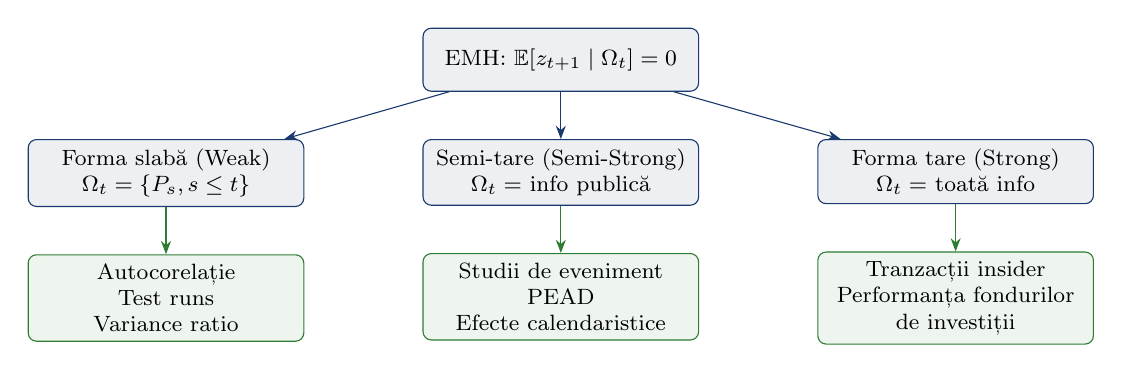
\begin{tikzpicture}[
    node distance=0.6cm and 1.5cm,
    every node/.style={font=\small, align=center},
    box/.style={draw=MainBlue, fill=MainBlue!8, rounded corners=3pt,
                minimum width=3.5cm, minimum height=0.8cm, font=\footnotesize},
    test/.style={draw=Forest, fill=Forest!8, rounded corners=3pt,
                minimum width=3.5cm, minimum height=0.8cm, font=\footnotesize}
]
\node[box] (emh) {EMH: $\E[z_{t+1}\mid\Omega_t]=0$};
\node[box, below left=of emh] (weak) {Forma slabă (Weak)\\$\Omega_t = \{P_s, s \leq t\}$};
\node[box, below=of emh] (semi) {Semi-tare (Semi-Strong)\\$\Omega_t =$ info publică};
\node[box, below right=of emh] (strong) {Forma tare (Strong)\\$\Omega_t =$ toată info};

\node[test, below=of weak] (t1) {Autocorelație\\Test runs\\Variance ratio};
\node[test, below=of semi] (t2) {Studii de eveniment\\PEAD\\Efecte calendaristice};
\node[test, below=of strong] (t3) {Tranzacții insider\\Performanța fondurilor\\de investiții};

\draw[-{Stealth}, MainBlue] (emh) -- (weak);
\draw[-{Stealth}, MainBlue] (emh) -- (semi);
\draw[-{Stealth}, MainBlue] (emh) -- (strong);
\draw[-{Stealth}, Forest] (weak) -- (t1);
\draw[-{Stealth}, Forest] (semi) -- (t2);
\draw[-{Stealth}, Forest] (strong) -- (t3);
\end{tikzpicture}
\end{center}
\end{cminipage}
\end{frame}

%#############################################################################
\section{Eficiența în formă slabă (Weak-Form)}
%#############################################################################

\slidelevel{Y3}
\begin{frame}{Testarea eficienței în formă slabă (Weak-Form)}
\begin{cminipage}{0.95\textwidth}
\begin{itemize}\setlength{\itemsep}{0pt}
    \item \textbf{Ipoteza nulă:} randamentele trecute nu conțin informație despre randamentele viitoare
    \item Dacă EMH în formă slabă (weak-form) este validă, randamentele ar trebui să fie serial necorelate:
$$\Corr(r_t, r_{t-k}) = 0, \quad \forall\, k \geq 1$$
\end{itemize}

\vspace{0.2cm}
\begin{block}{Principalele teste statistice}
\renewcommand{\arraystretch}{1.2}
\small
\begin{tabular}{lll}
\toprule
\textbf{Test} & \textbf{Ipoteza nulă} & \textbf{Metoda} \\
\midrule
Autocorelație & $\rho_k = 0$ pentru orice $k$ & Statistica Ljung--Box $Q$ \\
Test runs & Randamentele sunt aleatorii & Test neparametric de semn \\
Variance ratio & $\Var(r_t^{(q)}) = q \cdot \Var(r_t)$ & Lo--MacKinlay (1988) \\
Test ADF & Rădăcină unitară în prețuri & Augmented Dickey--Fuller \\
\bottomrule
\end{tabular}
\end{block}
\end{cminipage}
\quantlet{SFM\_ch3\_emh\_tests}{https://github.com/QuantLet/Stat_fin_markets/tree/master/Ch_03/SFM_ch3_emh_tests}
\end{frame}

\slidelevel{MSc}
\begin{frame}{Testul de autocorelație}
\begin{cminipage}{0.95\textwidth}
\begin{columns}[T]
\begin{column}{0.48\textwidth}
\begin{block}{Autocorelația eșantionului}
$$\hat{\rho}_k = \frac{\sum_{t=k+1}^{T}(r_t - \bar{r})(r_{t-k} - \bar{r})}{\sum_{t=1}^{T}(r_t - \bar{r})^2}$$
\end{block}

\begin{itemize}\setlength{\itemsep}{0pt}
    \item Sub $H_0$: $\hat{\rho}_k \sim \mathcal{N}(0, 1/T)$ aproximativ
    \item Se respinge dacă $|\hat{\rho}_k| > z_{\alpha/2}/\sqrt{T}$
\end{itemize}
\end{column}
\begin{column}{0.48\textwidth}
\begin{block}{Statistica Ljung--Box $Q$}
$$Q(m) = T(T+2)\sum_{k=1}^{m}\frac{\hat{\rho}_k^2}{T-k}$$
\end{block}

\begin{itemize}\setlength{\itemsep}{0pt}
    \item Testează ipoteza nulă compusă: $\rho_1 = \rho_2 = \cdots = \rho_m = 0$
    \item Sub $H_0$: $Q(m) \sim \chi^2(m)$
    \item Alegere tipică: $m = 10$ sau $m = 20$
\end{itemize}
\end{column}
\end{columns}

\vspace{0.2cm}
\begin{exampleblock}{Rezultat empiric}
\begin{itemize}\setlength{\itemsep}{0pt}
    \item Randamentele zilnice ale principalilor indici prezintă $\hat{\rho}_1 \approx 0{,}05$--$0{,}10$, mic dar statistic semnificativ (Lo \& MacKinlay, 1988). Economic nesemnificativ, dar contestă strict EMH în formă slabă.
\end{itemize}
\end{exampleblock}
\end{cminipage}
\end{frame}

\slidelevel{Y3}
\begin{frame}{Interpretarea graficului ACF}
\begin{cminipage}{0.95\textwidth}
\begin{columns}[T]
\begin{column}{0.55\textwidth}
\begin{itemize}\setlength{\itemsep}{0pt}
    \item Graficul ACF (\textit{autocorrelation function}) arată $\hat{\rho}_k$ pentru $k = 1, 2, \ldots, m$
    \item \textbf{Banda de încredere} 95\%: $\pm 1{,}96/\sqrt{T}$
    \item Bare care depășesc banda $\Rightarrow$ autocorelație semnificativă la lag-ul $k$
    \item \textbf{Piață eficientă:} toate barele ar trebui să fie în interiorul benzii (zgomot alb)
    \item \textbf{Randamente:} de regulă ACF aproape de zero --- eficiență aproximativă
    \item \textbf{Randamente pătratice} ($r_t^2$): ACF semnificativ pozitivă pe multe lag-uri $\Rightarrow$ clusterizare a volatilității (compatibilă cu EMH!)
\end{itemize}
\end{column}
\begin{column}{0.42\textwidth}
\begin{center}

\includegraphics[width=\textwidth]{ch3_emh_tests.pdf}
\end{center}
\end{column}
\end{columns}
\end{cminipage}
\quantlet{SFM\_ch3\_emh\_tests}{https://github.com/QuantLet/Stat_fin_markets/tree/master/Ch_03/SFM_ch3_emh_tests}
\end{frame}

\slidelevel{Y3}
\begin{frame}{Funcția de autocorelație: rezultate empirice}
\begin{cminipage}{0.95\textwidth}
\begin{center}
    
\includegraphics[width=0.55\textwidth]{ch3_emh_tests.pdf}
\end{center}
\begin{itemize}\setlength{\itemsep}{0pt}
    \item \textbf{Stânga:} ACF a randamentelor --- toate barele în interiorul benzii de încredere 95\%
    \item \textbf{Dreapta:} ACF a $r_t^2$ --- autocorelație semnificativă persistentă (clusterizare volatilitate)
\end{itemize}
\end{cminipage}
\quantlet{SFM\_ch3\_emh\_tests}{https://github.com/QuantLet/Stat_fin_markets/tree/master/Ch_03/SFM_ch3_emh_tests}
\end{frame}

\slidelevel{MSc}
\begin{frame}{Testul runs}
\begin{cminipage}{0.95\textwidth}
\begin{defn}[Run]
Un \textbf{run} este o secvență maximală consecutivă de randamente cu același semn. Ex.: $(+,+,-,-,-,+)$ are 3 run-uri.
\end{defn}

\begin{columns}[T]
\begin{column}{0.48\textwidth}
\begin{itemize}\setlength{\itemsep}{0pt}
    \item Fie $n_+$ = nr.\ randamente pozitive, $n_-$ = nr.\ randamente negative, $R$ = nr.\ run-uri
    \item Sub independență:
    $$\E[R] = \frac{2n_+n_-}{n_+ + n_-} + 1$$
    $$\Var(R) = \frac{2n_+n_-(2n_+n_- - n_+ - n_-)}{(n_++n_-)^2(n_++n_--1)}$$
\end{itemize}
\end{column}
\begin{column}{0.48\textwidth}
\begin{itemize}\setlength{\itemsep}{0pt}
    \item Statistica de test:
    $$Z = \frac{R - \E[R]}{\sqrt{\Var(R)}} \xrightarrow{d} \mathcal{N}(0,1)$$
    \item \textbf{Prea puține run-uri} $\Rightarrow$ impuls (autocorelație pozitivă)
    \item \textbf{Prea multe run-uri} $\Rightarrow$ reversie la medie (autocorelație negativă)
    \item Neparametric: nu necesită ipoteze distribuționale
\end{itemize}
\end{column}
\end{columns}
\end{cminipage}
\end{frame}

\slidelevel{MSc}
\begin{frame}{Testul variance ratio}
\begin{cminipage}{0.95\textwidth}
\begin{block}{Ideea cheie}
\begin{itemize}\setlength{\itemsep}{0pt}
    \item Dacă randamentele sunt iid, varianța randamentelor pe $q$ perioade ar trebui să crească liniar: $\Var(r_t(q)) = q \cdot \Var(r_t)$
\end{itemize}
\end{block}

\begin{columns}[T]
\begin{column}{0.50\textwidth}
\begin{itemize}\setlength{\itemsep}{0pt}
    \item \textbf{Raportul de varianță:}
    $$VR(q) = \frac{\Var(r_t(q))}{q \cdot \Var(r_t)} = 1 + 2\sum_{k=1}^{q-1}\!\left(1 - \frac{k}{q}\right)\rho_k$$
    \item $VR(q) = 1$: mers aleator (fără autocorelație)
    \item $VR(q) > 1$: autocorelație pozitivă (impuls)
    \item $VR(q) < 1$: autocorelație negativă (reversie la medie)
\end{itemize}
\end{column}
\begin{column}{0.46\textwidth}
\begin{itemize}\setlength{\itemsep}{0pt}
    \item \textbf{Lo--MacKinlay (1988):}
    $$Z(q) = \frac{VR(q) - 1}{\sqrt{\phi(q)}} \xrightarrow{d} \mathcal{N}(0,1)$$
    unde $\phi(q)$ este varianța asimptotică
    \item Versiune robustă la heteroscedasticitate disponibilă
    \item Tipic: $q = 2, 5, 10, 20$
\end{itemize}
\end{column}
\end{columns}
\end{cminipage}
\quantlet{SFM\_ch3\_variance\_ratio}{https://github.com/QuantLet/Stat_fin_markets/tree/master/Ch_03/SFM_ch3_variance_ratio}
\end{frame}

\slidelevel{MSc}
\begin{frame}{Testul ADF (Augmented Dickey--Fuller)}
\begin{cminipage}{0.95\textwidth}
\begin{block}{Modelul}
\begin{itemize}\setlength{\itemsep}{0pt}
    \item Se testează dacă seria de prețuri $\{P_t\}$ are rădăcină unitară (mers aleator):
$$\Delta P_t = \alpha + \beta t + \gamma P_{t-1} + \sum_{j=1}^{p} \delta_j \Delta P_{t-j} + \varepsilon_t$$
    \item $H_0$: $\gamma = 0$ (rădăcină unitară, serie nestaționară) vs.\ $H_1$: $\gamma < 0$ (staționaritate)
\end{itemize}
\end{block}

\begin{columns}[T]
\begin{column}{0.48\textwidth}
\begin{itemize}\setlength{\itemsep}{0pt}
    \item Statistica ADF \textbf{nu} are distribuție normală sub $H_0$ --- se folosesc tabele Dickey--Fuller
    \item Valori critice la 5\%: $\approx -2{,}86$ (fără trend), $\approx -3{,}41$ (cu trend)
    \item Se respinge $H_0$ dacă ADF $<$ valoarea critică
\end{itemize}
\end{column}
\begin{column}{0.48\textwidth}
\begin{itemize}\setlength{\itemsep}{0pt}
    \item \textbf{Rezultat tipic:} prețurile sunt $I(1)$ (ADF nu respinge $H_0$), dar log-randamentele sunt $I(0)$ (ADF respinge $H_0$)
    \item Consistent cu modelul mersului aleator pentru prețuri
    \item Lag-urile $p$ se aleg cu AIC sau BIC
\end{itemize}
\end{column}
\end{columns}
\end{cminipage}
\quantlet{SFM\_ch3\_emh\_tests}{https://github.com/QuantLet/Stat_fin_markets/tree/master/Ch_03/SFM_ch3_emh_tests}
\end{frame}

\slidelevel{MSc}
\begin{frame}{Variance ratio: rezultate empirice}
\begin{cminipage}{0.95\textwidth}
\small
\renewcommand{\arraystretch}{1.2}
\begin{center}
\begin{tabular}{lccccl}
\toprule
\textbf{Piață} & $VR(2)$ & $VR(5)$ & $VR(10)$ & $VR(20)$ & \textbf{Interpretare} \\
\midrule
S\&P 500 & 1,05 & 1,04 & 0,99 & 0,95 & Impuls scurt, reversie lungă \\
FTSE 100 & 1,03 & 1,01 & 0,97 & 0,92 & Reversie moderată \\
BTC-USD & 1,02 & 0,98 & 0,94 & 0,88 & Reversie pe orizonturi lungi \\
BET & 1,12 & 1,18 & 1,10 & 1,01 & Impuls puternic (ineficient) \\
\bottomrule
\end{tabular}
\end{center}

\vspace{0.2cm}
\begin{itemize}\setlength{\itemsep}{0pt}
    \item Piețe dezvoltate: $VR \approx 1$ la majoritatea orizonturilor $\Rightarrow$ aproximativ eficiente
    \item Piețe emergente (BET): deviații mai mari $\Rightarrow$ potențială ineficiență
    \item Crypto: eficiență ridicată pe termen scurt, reversie la medie pe termen lung
    \item \textbf{Tipar:} VR $> 1$ la orizonturi scurte, VR $< 1$ la orizonturi lungi --- impuls pe termen scurt și reversie la medie pe termen lung (Poterba \& Summers, 1988)
\end{itemize}
\end{cminipage}
\end{frame}

\slidelevel{MSc}
\begin{frame}{Variance ratio: grafic comparativ}
\begin{cminipage}{0.95\textwidth}
\begin{center}
    
\includegraphics[width=0.55\textwidth]{ch3_variance_ratio.pdf}
\end{center}
\begin{itemize}\setlength{\itemsep}{0pt}
    \item $VR(q)$ pentru $q = 2, 5, 10, 20$ cu benzi de încredere 95\%
    \item Piețe dezvoltate: $VR \approx 1$; piețe emergente: deviații semnificative
\end{itemize}
\end{cminipage}
\quantlet{SFM\_ch3\_variance\_ratio}{https://github.com/QuantLet/Stat_fin_markets/tree/master/Ch_03/SFM_ch3_variance_ratio}
\end{frame}

\slidelevel{PhD}
\begin{frame}{Variance ratio mobil și eficiența variabilă în timp}
\begin{cminipage}{0.95\textwidth}
\footnotesize
\begin{itemize}\setlength{\itemsep}{0pt}
    \item \textbf{Variance ratio mobil:} $VR(q)$ pe fereastră mobilă de 500 zile; $|VR(q) - 1|$ = \textbf{indice de eficiență}
\end{itemize}

\vspace{0.05cm}
\begin{center}

\includegraphics[width=0.70\textwidth]{ch3_variance_ratio.pdf}
\end{center}

\vspace{0.02cm}
\begin{itemize}\setlength{\itemsep}{0pt}
    \item În crize (2008, 2020), $|VR - 1|$ crește abrupt $\Rightarrow$ ineficiență temporară
    \item BET: nivel de bază mai ridicat $\Rightarrow$ piață mai puțin eficientă structural
    \item Între crize, eficiența este restabilită --- consistent cu AMH
\end{itemize}
\end{cminipage}
\quantlet{SFM\_ch3\_variance\_ratio}{https://github.com/QuantLet/Stat_fin_markets/tree/master/Ch_03/SFM_ch3_variance_ratio}
\end{frame}

\slidelevel{MSc}
\begin{frame}{Studiu de caz: Eficiența EMH pe S\&P 500}
\begin{cminipage}{0.95\textwidth}
\small
\begin{block}{Date: S\&P 500, randamente zilnice, 2000--2025 ($T \approx 6300$)}
\begin{itemize}\setlength{\itemsep}{0pt}
    \item Sursa: Yahoo Finance via \texttt{yfinance}
\end{itemize}
\end{block}

\renewcommand{\arraystretch}{1.15}
\begin{center}
\scriptsize
\begin{tabular}{llll}
\toprule
\textbf{Test} & \textbf{Statistică} & \textbf{$p$-value} & \textbf{Decizie} \\
\midrule
Ljung--Box $Q(10)$ & $Q = 18{,}7$ & 0,044 & Respingere marginală la 5\% \\
Ljung--Box $Q(20)$ & $Q = 28{,}3$ & 0,102 & Non-respingere la 5\% \\
Test runs & $Z = -1{,}82$ & 0,069 & Non-respingere marginală \\
VR(2) Lo--MacKinlay & $Z = 2{,}41$ & 0,016 & Respingere la 5\% \\
VR(5) Lo--MacKinlay & $Z = 1{,}34$ & 0,181 & Non-respingere \\
ADF (prețuri) & $\tau = -1{,}23$ & 0,66 & Rădăcină unitară (așteptat) \\
ADF (randamente) & $\tau = -56{,}1$ & $< 0{,}001$ & Staționare (așteptat) \\
\bottomrule
\end{tabular}
\end{center}

\vspace{0.1cm}
\begin{alertblock}{Concluzie}
\begin{itemize}\setlength{\itemsep}{0pt}
    \item S\&P 500 este \textbf{aproximativ eficient}: autocorelație statistică slabă la lag 1, dar economic nesemnificativă. Costurile de tranzacționare elimină orice profit potențial.
\end{itemize}
\end{alertblock}
\end{cminipage}
\end{frame}

\slidelevel{MSc}
\begin{frame}{Eficiența pe piețe emergente: Indicele BET}
\begin{cminipage}{0.95\textwidth}
\small
\begin{columns}[T]
\begin{column}{0.48\textwidth}
\begin{block}{Rezultate BET (2005--2025)}
\begin{itemize}\setlength{\itemsep}{0pt}
    \item $\hat{\rho}_1 = 0{,}11$ (semnificativ la 1\%)
    \item Ljung--Box $Q(10) = 42{,}5$ ($p < 0{,}001$)
    \item $VR(2) = 1{,}12$, $VR(5) = 1{,}18$
    \item Test runs: $Z = -3{,}24$ ($p = 0{,}001$)
    \item Exponent Hurst: $H \approx 0{,}58$
\end{itemize}
\end{block}
\begin{itemize}\setlength{\itemsep}{0pt}
    \item Autocorelație semnificativă $\Rightarrow$ eficiența slabă este respinsă
    \item Cauzele posibile: lichiditate redusă, costuri de tranzacționare mari, tranzacții nesincronizate
\end{itemize}
\end{column}
\begin{column}{0.48\textwidth}
\begin{block}{Comparație piețe emergente}
\renewcommand{\arraystretch}{1.1}
\scriptsize
\begin{tabular}{lccc}
\toprule
\textbf{Piață} & $\hat{\rho}_1$ & $VR(5)$ & $H$ \\
\midrule
BET (România) & 0,11 & 1,18 & 0,58 \\
WIG (Polonia) & 0,06 & 1,08 & 0,54 \\
BUX (Ungaria) & 0,05 & 1,05 & 0,53 \\
BIST (Turcia) & 0,04 & 1,03 & 0,52 \\
\midrule
S\&P 500 & 0,02 & 1,04 & 0,52 \\
\bottomrule
\end{tabular}
\end{block}
\begin{itemize}\setlength{\itemsep}{0pt}
    \item Piețele emergente din Europa Centrală și de Est sunt mai puțin eficiente decât piețele dezvoltate
    \item BET prezintă cea mai mare abatere de la eficiență
\end{itemize}
\end{column}
\end{columns}
\end{cminipage}
\quantlet{SFM\_ch3\_efficiency\_comparison}{https://github.com/QuantLet/Stat_fin_markets/tree/master/Ch_03/SFM_ch3_efficiency_comparison}
\end{frame}

%--- Python code slide: Autocorelație + Ljung-Box ---
\slidelevel{MSc}
\begin{frame}[fragile]{Python: Autocorelație și testul Ljung--Box}
\begin{cminipage}{0.95\textwidth}
\begin{lstlisting}
import yfinance as yf
import numpy as np
from statsmodels.stats.diagnostic import acorr_ljungbox
from statsmodels.tsa.stattools import acf

# Descarca date S&P 500
sp = yf.download("^GSPC", start="2000-01-01", end="2025-01-01")
ret = np.log(sp["Close"] / sp["Close"].shift(1)).dropna()

# Autocorelatie esantion
rho = acf(ret, nlags=20, fft=True)
print(f"rho_1 = {rho[1]:.4f}, rho_5 = {rho[5]:.4f}")

# Testul Ljung-Box
lb = acorr_ljungbox(ret, lags=[10, 20], return_df=True)
print(lb)
# Q(10)=18.7 (p=0.044), Q(20)=28.3 (p=0.102)
\end{lstlisting}
\end{cminipage}
\quantlet{SFM\_ch3\_emh\_tests}{https://github.com/QuantLet/Stat_fin_markets/tree/master/Ch_03/SFM_ch3_emh_tests}
\end{frame}

%--- Python code slide: Variance ratio ---
\slidelevel{MSc}
\begin{frame}[fragile]{Python: Testul variance ratio pe S\&P 500}
\begin{cminipage}{0.95\textwidth}
\begin{lstlisting}
import numpy as np

def variance_ratio(returns, q):
    """Calculeaza VR(q) si statistica Z Lo-MacKinlay."""
    T = len(returns)
    mu = returns.mean()
    # Varianta pe 1 perioada
    var1 = np.sum((returns - mu)**2) / (T - 1)
    # Randamente pe q perioade
    ret_q = np.array([returns[i:i+q].sum()
                      for i in range(T - q + 1)])
    varq = np.sum((ret_q - q * mu)**2) / (T - q)
    vr = varq / (q * var1)
    # Varianta asimptotica (sub homoscedasticitate)
    phi = 2 * (2*q - 1) * (q - 1) / (3 * q * T)
    z = (vr - 1) / np.sqrt(phi)
    return vr, z

for q in [2, 5, 10, 20]:
    vr, z = variance_ratio(ret.values, q)
    print(f"VR({q:2d}) = {vr:.4f},  Z = {z:+.3f}")
\end{lstlisting}
\end{cminipage}
\end{frame}

%=============================================================================
% SECȚIUNEA A: Teste extinse de mers aleator
%=============================================================================

\slidelevel{MSc}
\begin{frame}[shrink=3]{Testul ADF: Formulare}
\begin{cminipage}{0.95\textwidth}
\footnotesize
\begin{block}{Ecuația de regresie ADF}
\begin{itemize}\setlength{\itemsep}{0pt}
    \item Augmented Dickey--Fuller cu trend:
    $\Delta P_t = \alpha + \beta t + \gamma P_{t-1} + \sum_{j=1}^{p} \delta_j \Delta P_{t-j} + \varepsilon_t$
    \item $H_0$: $\gamma = 0$ (rădăcină unitară) vs.\ $H_1$: $\gamma < 0$ (staționaritate)
\end{itemize}
\end{block}

\begin{columns}[T]
\begin{column}{0.48\textwidth}
\begin{itemize}\setlength{\itemsep}{0pt}
    \item \textbf{Selecția lag-urilor $p$:}
    \item AIC: $\text{AIC}(p) = \ln\hat{\sigma}^2_p + \frac{2p}{T}$
    \item BIC: $\text{BIC}(p) = \ln\hat{\sigma}^2_p + \frac{p\ln T}{T}$
    \item BIC preferă modele mai parsimonioase
    \item Alternativă: general-to-specific (de la $p_{\max}$, se elimină lag-uri nesemnificative)
\end{itemize}
\end{column}
\begin{column}{0.48\textwidth}
\begin{itemize}\setlength{\itemsep}{0pt}
    \item \textbf{Valori critice MacKinnon (1996):}
    \item 1\%: $-3{,}43$; 5\%: $-2{,}86$; 10\%: $-2{,}57$ (fără trend)
    \item 1\%: $-3{,}96$; 5\%: $-3{,}41$; 10\%: $-3{,}13$ (cu trend)
    \item Se respinge $H_0$ dacă $\tau_{\text{ADF}} <$ valoarea critică
    \item \textbf{Interpretare EMH:} prețurile $I(1)$ $\Rightarrow$ mers aleator; randamentele $I(0)$ $\Rightarrow$ consistent
\end{itemize}
\end{column}
\end{columns}
\end{cminipage}
\quantlet{SFM\_ch3\_emh\_tests}{https://github.com/QuantLet/Stat_fin_markets/tree/master/Ch_03/SFM_ch3_emh_tests}
\end{frame}

\slidelevel{MSc}
\begin{frame}{Testele Phillips--Perron și KPSS}
\begin{cminipage}{0.95\textwidth}
\small
\begin{columns}[T]
\begin{column}{0.48\textwidth}
\begin{block}{Phillips--Perron (PP)}
\begin{itemize}\setlength{\itemsep}{0pt}
    \item Corectează neparametric autocorelația reziduurilor
    \item Nu adaugă lag-uri $\Delta P_{t-j}$; în schimb, ajustează statistica $t$ folosind estimatorul Newey--West
    \item $H_0$: rădăcină unitară (ca ADF)
    \item Avantaj: robust la heteroscedasticitate și autocorelație de formă necunoscută
\end{itemize}
\end{block}
\end{column}
\begin{column}{0.48\textwidth}
\begin{block}{Kwiatkowski--Phillips--Schmidt--Shin, KPSS (1992)}
\begin{itemize}\setlength{\itemsep}{0pt}
    \item \textbf{Inversează ipotezele:}
    \item $H_0$: seria este staționară
    \item $H_1$: seria are rădăcină unitară
    \item Statistica: $\eta = T^{-2}\sum_{t=1}^{T} S_t^2 / \hat{\sigma}^2_{LR}$
    \item $\hat{\sigma}^2_{LR}$ = varianța pe termen lung (Bartlett kernel)
\end{itemize}
\end{block}
\end{column}
\end{columns}

\vspace{0.15cm}
\renewcommand{\arraystretch}{1.1}
\begin{center}
\scriptsize
\begin{tabular}{llll}
\toprule
\textbf{Test} & \textbf{$H_0$} & \textbf{$H_1$} & \textbf{Utilizare EMH} \\
\midrule
ADF & Rădăcină unitară & Staționaritate & Non-respingere $\Rightarrow$ mers aleator \\
PP & Rădăcină unitară & Staționaritate & Robust la heterosced. \\
KPSS & Staționaritate & Rădăcină unitară & Respingere $\Rightarrow$ mers aleator \\
\bottomrule
\end{tabular}
\end{center}
\end{cminipage}
\end{frame}

\slidelevel{PhD}
\begin{frame}{Analiza spectrală pentru eficiența în formă slabă (Weak-Form)}
\begin{cminipage}{0.95\textwidth}
\footnotesize
\begin{block}{Densitatea spectrală a randamentelor}
\begin{itemize}\setlength{\itemsep}{0pt}
    \item Descompune varianța pe frecvențe: $f(\omega) = \frac{1}{2\pi}\left[\gamma_0 + 2\sum_{k=1}^{\infty}\gamma_k \cos(\omega k)\right]$
    \item Zgomot alb: $f(\omega) = \sigma^2/(2\pi)$ --- spectru \textbf{plat} (constant)
\end{itemize}
\end{block}
\vspace{-0.1cm}
\begin{columns}[T]
\begin{column}{0.48\textwidth}
\begin{itemize}\setlength{\itemsep}{0pt}
    \item \textbf{Testul Bartlett (1955):}
    \item Compară periodograma cumulată cu distribuția uniformă
    \item Statistica Kolmogorov--Smirnov pe spectrul cumulat
    \item $H_0$: spectru plat (zgomot alb)
    \item Respingere $\Rightarrow$ dependență serial la anumite frecvențe
\end{itemize}
\end{column}
\begin{column}{0.48\textwidth}
\begin{itemize}\setlength{\itemsep}{0pt}
    \item \textbf{Interpretare EMH:}
    \item Spectru plat $\Rightarrow$ nicio frecvență dominantă $\Rightarrow$ EMH consistent
    \item Pic la frecvențe joase $\Rightarrow$ memorie lungă (anti-EMH)
    \item Pic la frecvențe înalte $\Rightarrow$ microstructură / bouncing
    \item Avantaj: detectează tipare periodice invizibile în ACF
\end{itemize}
\end{column}
\end{columns}
\end{cminipage}
\end{frame}

\slidelevel{Y3}
\begin{frame}{Reguli de filtrare și tranzacționare tehnică (Filter Rules)}
\begin{cminipage}{0.95\textwidth}
\small
\begin{columns}[T]
\begin{column}{0.48\textwidth}
\begin{block}{Regulile Alexander (1961)}
\begin{itemize}\setlength{\itemsep}{0pt}
    \item Cumpără dacă prețul crește cu $x\%$ de la un minim local
    \item Vinde dacă prețul scade cu $x\%$ de la un maxim local
    \item Filtre tipice: $x = 0{,}5\%$, $1\%$, $2\%$, $5\%$
    \item Fama \& Blume (1966): filtrele mici generează profit brut, dar \textbf{nu} după costuri de tranzacționare
\end{itemize}
\end{block}
\end{column}
\begin{column}{0.48\textwidth}
\begin{block}{Medie mobilă crossover}
\begin{itemize}\setlength{\itemsep}{0pt}
    \item Cumpără când MA scurtă $>$ MA lungă
    \item Vinde când MA scurtă $<$ MA lungă
    \item Exemple: MA(50) vs MA(200) (,,Golden Cross'' / ,,Death Cross'')
    \item Brock, Lakonishok \& LeBaron (1992): profitabile pe date pre-1990
    \item Post-1990: profitabilitatea dispare $\Rightarrow$ piața se adaptează
\end{itemize}
\end{block}
\end{column}
\end{columns}

\vspace{0.15cm}
\begin{alertblock}{Concluzie}
\begin{itemize}\setlength{\itemsep}{0pt}
    \item Majoritatea strategiilor de analiză tehnică \textbf{eșuează} după includerea costurilor de tranzacționare, slippage și impactul de piață. Rezultat consistent cu EMH în formă slabă (weak-form).
\end{itemize}
\end{alertblock}
\end{cminipage}
\end{frame}

\slidelevel{MSc}
\begin{frame}[fragile]{Python: Teste de rădăcină unitară (Unit Root)}
\begin{cminipage}{0.95\textwidth}
\begin{lstlisting}
import yfinance as yf, numpy as np
from statsmodels.tsa.stattools import adfuller, kpss

sp = yf.download("^GSPC", start="2000-01-01", end="2025-01-01")
prices = sp["Close"].dropna()
ret = np.log(prices / prices.shift(1)).dropna()

# Test ADF pe preturi (asteptam non-respingere = radacina unitara)
adf_p = adfuller(prices, maxlag=20, autolag="BIC")
print(f"ADF preturi:  stat={adf_p[0]:.3f}, p={adf_p[1]:.4f}")

# Test ADF pe randamente (asteptam respingere = stationaritate)
adf_r = adfuller(ret, maxlag=20, autolag="BIC")
print(f"ADF randamente: stat={adf_r[0]:.3f}, p={adf_r[1]:.6f}")

# Test KPSS pe randamente (H0: stationaritate)
kpss_r = kpss(ret, regression="c", nlags="auto")
print(f"KPSS randamente: stat={kpss_r[0]:.4f}, p={kpss_r[1]:.4f}")
# ADF preturi: stat=-1.23, p=0.66  (radacina unitara)
# ADF randamente: stat=-56.1, p<0.001  (stationare)
# KPSS randamente: stat=0.12, p>0.10  (stationare)
\end{lstlisting}
\end{cminipage}
\quantlet{SFM\_ch3\_emh\_tests}{https://github.com/QuantLet/Stat_fin_markets/tree/master/Ch_03/SFM_ch3_emh_tests}
\end{frame}

%#############################################################################
\section{Eficiența în formă semi-tare (Semi-Strong)}
%#############################################################################

\slidelevel{Y3}
\begin{frame}{Testarea eficienței semi-tare: studii de eveniment}
\begin{cminipage}{0.95\textwidth}
\small
\begin{block}{Metodologie}
\begin{itemize}\setlength{\itemsep}{0pt}
    \item Se măsoară reacția prețului la un eveniment informațional public (câștiguri, M\&A, dividende)
    \item Dacă EMH semi-tare este validă: prețul se ajustează \textbf{imediat} și \textbf{complet} la știre
\end{itemize}
\end{block}

\begin{columns}[T]
\begin{column}{0.48\textwidth}
\begin{itemize}\setlength{\itemsep}{0pt}
    \item \textbf{Pasul 1:} Estimarea rand.\ normale pe fereastra $[-250, -11]$:
    $R_{i,t} = \alpha_i + \beta_i R_{m,t} + \varepsilon_{i,t}$
    \item \textbf{Pasul 2:} Randamentele anormale pe $[-10, +10]$:
    $AR_{i,t} = R_{i,t} - (\hat{\alpha}_i + \hat{\beta}_i R_{m,t})$
\end{itemize}
\end{column}
\begin{column}{0.48\textwidth}
\begin{itemize}\setlength{\itemsep}{0pt}
    \item \textbf{Pasul 3:} Randamentul anormal cumulat:
    $CAR_i(\tau_1, \tau_2) = \sum_{t=\tau_1}^{\tau_2} AR_{i,t}$
    \item \textbf{Pasul 4:} Media pe $N$ evenimente:
    $\overline{CAR}(\tau_1, \tau_2) = \frac{1}{N}\sum_{i=1}^{N} CAR_i$
    \item Test: $t = \overline{CAR} / (\hat{\sigma}_{CAR}/\sqrt{N})$
\end{itemize}
\end{column}
\end{columns}
\end{cminipage}
\end{frame}

\slidelevel{Y3}
\begin{frame}{Studiu de eveniment: trei scenarii}
\begin{cminipage}{0.95\textwidth}
\begin{center}

\includegraphics[width=0.65\textwidth]{ch3_event_study.pdf}
\end{center}

\vspace{0.2cm}
\begin{itemize}\setlength{\itemsep}{0pt}
    \item \textcolor{Forest}{\textbf{Eficient:}} ajustare instantanee, fără derivă post-eveniment
    \item \textcolor{Crimson}{\textbf{Suprareacție:}} depășire inițială, apoi inversare (De Bondt \& Thaler, 1985)
    \item \textcolor{MainBlue}{\textbf{Subreacție:}} ajustare lentă, derivă post-eveniment (Post-Earnings Announcement Drift, PEAD --- Ball \& Brown, 1968)
\end{itemize}
\end{cminipage}
\end{frame}

\slidelevel{MSc}
\begin{frame}{Deriva post-anunț de câștiguri (PEAD)}
\begin{cminipage}{0.95\textwidth}
\begin{columns}[T]
\begin{column}{0.55\textwidth}
\begin{itemize}\setlength{\itemsep}{0pt}
    \item După surprize privind câștigurile, prețurile acțiunilor continuă să derive în direcția surprizei timp de 60--90 de zile
    \item Una dintre cele mai puternice și persistente anomalii, documentată din Ball \& Brown (1968)
    \item \textbf{Surpriza de câștiguri} --- Standardized Unexpected Earnings (SUE):
    $$SUE_t = \frac{EPS_t - \E[EPS_t]}{\sigma_{EPS}}$$
    \item Acțiunile din decila superioară SUE depășesc decila inferioară cu $\sim$4\% pe trimestru
    \item Supraviețuiește costurilor de tranzacționare în multe studii
\end{itemize}
\end{column}
\begin{column}{0.42\textwidth}
\begin{alertblock}{Provocare la adresa EMH semi-tare}
\begin{itemize}\setlength{\itemsep}{0pt}
    \item PEAD implică faptul că prețurile \textbf{nu} se ajustează complet la informația publică privind câștigurile
    \item Fama (1998): ,,bunicul evenimentelor de subreacție''
    \item Persistă pe diverse piețe, perioade și metodologii
\end{itemize}
\end{alertblock}
\end{column}
\end{columns}
\end{cminipage}
\end{frame}

%--- Python code slide: Event study ---
\slidelevel{MSc}
\begin{frame}[fragile]{Python: Simulare event study}
\begin{cminipage}{0.95\textwidth}
\begin{lstlisting}
import numpy as np
np.random.seed(42)
T_est, T_evt, N = 240, 21, 50  # estimare, eveniment, nr
alpha, beta = 0.0002, 1.1
car_all = []
for _ in range(N):
    r_m = np.random.normal(0.0003, 0.01, T_est + T_evt)
    eps = np.random.normal(0, 0.015, T_est + T_evt)
    r_i = alpha + beta * r_m + eps
    r_i[T_est] += 0.03  # surpriza de 3% la t=0
    rm_est, ri_est = r_m[:T_est], r_i[:T_est]
    b = np.cov(ri_est, rm_est)[0,1] / np.var(rm_est)
    a = ri_est.mean() - b * rm_est.mean()
    ar = r_i[T_est:] - (a + b * r_m[T_est:])  # AR
    car_all.append(np.cumsum(ar))

car_mean = np.mean(car_all, axis=0)
se = np.std([c[-1] for c in car_all]) / np.sqrt(N)
print(f"CAR(-10,+10) = {car_mean[-1]:.4f}, t = {car_mean[-1]/se:.2f}")
\end{lstlisting}
\end{cminipage}
\quantlet{SFM\_ch3\_event\_study}{https://github.com/QuantLet/Stat_fin_markets/tree/master/Ch_03/SFM_ch3_event_study}
\end{frame}

\slidelevel{MSc}
\begin{frame}{Studiu de eveniment: rezultate empirice}
\begin{cminipage}{0.95\textwidth}
\begin{center}

\includegraphics[width=0.55\textwidth]{ch3_event_study.pdf}
\end{center}
\begin{itemize}\setlength{\itemsep}{0pt}
    \item Randamentul anormal cumulat (CAR) arată ajustarea prețului în jurul evenimentului ($t = 0$)
    \item Deriva post-anunț vizibilă: piața nu se ajustează complet și imediat
\end{itemize}
\end{cminipage}
\quantlet{SFM\_ch3\_event\_study}{https://github.com/QuantLet/Stat_fin_markets/tree/master/Ch_03/SFM_ch3_event_study}
\end{frame}

%#############################################################################
\section{Eficiența în formă tare (Strong-Form)}
%#############################################################################

\slidelevel{Y3}
\begin{frame}{Testarea eficienței în formă tare (Strong-Form)}
\begin{cminipage}{0.95\textwidth}
\begin{block}{Întrebare}
\begin{itemize}\setlength{\itemsep}{0pt}
    \item Pot investitorii cu informații \textbf{private} să obțină randamente anormale?
\end{itemize}
\end{block}

\begin{columns}[T]
\begin{column}{0.48\textwidth}
\begin{itemize}\setlength{\itemsep}{0pt}
    \item \textbf{Evidențe din insider trading:}
    \item Insiderii corporativi obțin $\sim$5--8\% randamente anormale din tranzacțiile lor (Jeng et al., 2003)
    \item Insiderii cumpără înainte de creșteri de preț, vând înainte de scăderi
    \item Raportările SEC (Formularul 4) arată tipare sistematice
    \item $\Rightarrow$ EMH în formă tare (strong-form) este \textcolor{Crimson}{\textbf{respinsă}}
\end{itemize}
\end{column}
\begin{column}{0.48\textwidth}
\begin{itemize}\setlength{\itemsep}{0pt}
    \item \textbf{Evidențe din performanța managerilor de fonduri:}
    \item Jensen (1968): fondurile mutuale nu bat piața după comisioane
    \item Carhart (1997): persistența randamentelor fondurilor se explică prin momentum, nu prin abilitate
    \item SPIVA (2024): 92\% din fondurile US large-cap subperformează S\&P 500 pe 15 ani
    \item $\Rightarrow$ Managerii profesioniști ca grup \textbf{nu} au informații private
\end{itemize}
\end{column}
\end{columns}
\end{cminipage}
\end{frame}

\slidelevel{MSc}
\begin{frame}{Paradoxul Grossman--Stiglitz}
\begin{cminipage}{0.95\textwidth}
\small
\begin{thm}[Grossman \& Stiglitz, 1980]
Dacă piețele sunt perfect eficiente, niciun investitor nu are stimulente să cheltuiască resurse pentru achiziția de informații. Dar dacă nimeni nu achiziționează informații, prețurile nu le pot reflecta. Prin urmare, piețele perfect eficiente sunt o imposibilitate.
\end{thm}

\vspace{0.1cm}
\begin{columns}[T]
\begin{column}{0.48\textwidth}
\begin{itemize}\setlength{\itemsep}{0pt}
    \item \textbf{Rezolvare:} piețele trebuie să fie ,,eficient ineficiente''
    \item Prețurile sunt \textit{aproape} eficiente --- suficient de apropiate încât majoritatea nu pot profita, dar cu suficiente deviații pentru a recompensa traderii informați
    \item Gradul de eficiență depinde de:
    \begin{itemize}\setlength{\itemsep}{0pt}
        \item Costul achiziției de informații
        \item Numărul de traderi informați
        \item Lichiditatea pieței
    \end{itemize}
\end{itemize}
\end{column}
\begin{column}{0.48\textwidth}
\begin{center}
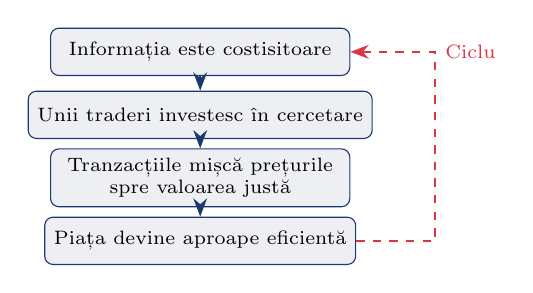
\begin{tikzpicture}[
    every node/.style={font=\small, align=center},
    box/.style={draw=MainBlue, fill=MainBlue!8, rounded corners=3pt,
                minimum width=3.8cm, minimum height=0.6cm, font=\scriptsize}
]
\node[box] (a) at (0,2.6) {Informația este costisitoare};
\node[box] (b) at (0,1.8) {Unii traderi investesc în cercetare};
\node[box] (c) at (0,1.0) {Tranzacțiile mișcă prețurile\\spre valoarea justă};
\node[box] (d) at (0,0.2) {Piața devine aproape eficientă};
\draw[-{Stealth}, MainBlue, thick] (a) -- (b);
\draw[-{Stealth}, MainBlue, thick] (b) -- (c);
\draw[-{Stealth}, MainBlue, thick] (c) -- (d);
\draw[-{Stealth}, Crimson, thick, dashed] (d.east) -- ++(1.0,0) |- (a.east) node[midway, right, font=\scriptsize, Crimson] {Ciclu};
\end{tikzpicture}
\end{center}
\end{column}
\end{columns}
\end{cminipage}
\end{frame}

%#############################################################################
\section{Anomalii de piață}
%#############################################################################

\slidelevel{Y3}
\begin{frame}{Anomalii calendaristice}
\begin{cminipage}{0.95\textwidth}
\small
\renewcommand{\arraystretch}{1.2}
\begin{center}
\scriptsize
\begin{tabular}{lll}
\toprule
\textbf{Anomalie} & \textbf{Descriere} & \textbf{Status actual} \\
\midrule
Efectul ianuarie & Acțiunile mici au randamente mai mari în ianuarie & Slăbit semnificativ de la descoperire \\
Efectul luni & Randamentele sunt mai mici lunea & Dispărut în mare parte \\
Schimbarea de lună & Rand.\ mai mari în ultimele și primele 3 zile & Încă prezent, legat de fluxuri salariale \\
Efectul de sărbătoare & Randamentele înainte de sărbători sunt mai mari & Persistă slab \\
Halloween & ,,Vinde în mai și pleacă'' & Evidență mixtă, dep.\ de regiune \\
\bottomrule
\end{tabular}
\end{center}

\vspace{0.2cm}
\begin{alertblock}{Biasul publicării și declinul anomaliilor}
\begin{itemize}\setlength{\itemsep}{0pt}
    \item Multe anomalii slăbesc sau dispar după publicare --- consistent cu EMH! Traderii de arbitraj (\textit{arbitrageurs}) elimină greșelile de preț odată ce devin cunoscute (McLean \& Pontiff, 2016).
\end{itemize}
\end{alertblock}
\end{cminipage}
\end{frame}

\slidelevel{Y3}
\begin{frame}{Anomalii transversale}
\begin{cminipage}{0.95\textwidth}
\small
\begin{columns}[T]
\begin{column}{0.48\textwidth}
\begin{block}{Efectul de valoare}
\begin{itemize}\setlength{\itemsep}{0pt}
    \item Acțiuni cu B/M ridicat au randamente superioare (Fama \& French, 1993)
    \item Factorul High Minus Low (HML): $\sim$4\% pe an istoric
    \item Primă de risc sau eroare de preț?
\end{itemize}
\end{block}

\begin{block}{Efectul de dimensiune}
\begin{itemize}\setlength{\itemsep}{0pt}
    \item Acțiuni cu capitalizare mică au randamente superioare (Banz, 1981)
    \item Factorul Small Minus Big (SMB): $\sim$2\% pe an; slăbit de la descoperire
\end{itemize}
\end{block}
\end{column}
\begin{column}{0.48\textwidth}
\begin{block}{Momentum}
\begin{itemize}\setlength{\itemsep}{0pt}
    \item Câștigătorii continuă să câștige pe 3--12 luni (Jegadeesh \& Titman, 1993)
    \item Factorul Winners Minus Losers (WML): $\sim$8\% pe an; prăbușiri ocazionale (2009)
    \item Cea mai dificilă anomalie de explicat rațional
\end{itemize}
\end{block}

\begin{block}{Volatilitate scăzută}
\begin{itemize}\setlength{\itemsep}{0pt}
    \item Acțiuni cu vol.\ scăzută au rand.\ ajustate la risc superioare
    \item Contrazice relația risc-randament din CAPM
    \item Explicații: constrângeri de levier, preferințe loterie
\end{itemize}
\end{block}
\end{column}
\end{columns}
\end{cminipage}
\end{frame}

\slidelevel{Y3}
\begin{frame}{Anomalii extinse: De ce persistă unele?}
\begin{cminipage}{0.95\textwidth}
\begin{columns}[T]
\begin{column}{0.48\textwidth}
\begin{block}{Limita arbitrajului (Shleifer \& Vishny, 1997)}
\begin{itemize}\setlength{\itemsep}{0pt}
    \item Riscul de model: eroarea de preț se poate agrava
    \item Riscul de lichiditate: active greu de vândut rapid
    \item Costuri de tranzacționare: spread, comisioane, impact
    \item Riscul de finanțare: margin call forțează închiderea
    \item LTCM (1998): aveau dreptate pe termen lung, dar au dat faliment pe termen scurt
\end{itemize}
\end{block}
\end{column}
\begin{column}{0.48\textwidth}
\begin{block}{De ce dispar anomaliile?}
\begin{itemize}\setlength{\itemsep}{0pt}
    \item McLean \& Pontiff (2016): randamentele anomaliilor scad cu 58\% după publicare
    \item Capital-ul atras de anomalie elimină profitul
    \item Îmbunătățiri tehnologice (High-Frequency Trading, HFT) accelerează procesul
    \item Anomaliile care supraviețuiesc sunt cele greu de arbitrajat (iliciditate, costuri mari)
\end{itemize}
\end{block}

\begin{exampleblock}{Implicație}
\begin{itemize}\setlength{\itemsep}{0pt}
    \item Declinul anomaliilor post-publicare este \textbf{în sine o dovadă} pentru EMH
\end{itemize}
\end{exampleblock}
\end{column}
\end{columns}
\end{cminipage}
\end{frame}

\slidelevel{PhD}
\begin{frame}{Grădina zoologică a factorilor (Factor Zoo)}
\begin{cminipage}{0.95\textwidth}
\small
\begin{itemize}\setlength{\itemsep}{0pt}
    \item Harvey, Liu \& Zhu (2016): peste \textbf{300} de factori publicați care pretind că prezic randamentele
    \item Mulți sunt probabil descoperiri false din cauza data mining-ului și $p$-hacking-ului
    \item Hou, Xue \& Zhang (2020): majoritatea anomaliilor nu supraviețuiesc replicării cu corecții adecvate
\end{itemize}

\vspace{0.1cm}
\renewcommand{\arraystretch}{1.1}
\begin{center}
\footnotesize
\begin{tabular}{lccl}
\toprule
\textbf{Factor} & \textbf{$t$-stat (original)} & \textbf{$t$-stat (replicat)} & \textbf{Status} \\
\midrule
Valoare (HML) & 3,07 & 2,83 & Robust \\
Momentum (WML) & 4,71 & 3,92 & Robust \\
Dimensiune (SMB) & 2,28 & 1,31 & Slăbit \\
Accruals & 4,33 & 0,89 & Non-robust \\
Creșterea activelor & 5,07 & 1,61 & Slăbit \\
\bottomrule
\end{tabular}
\end{center}

\vspace{0.1cm}
\begin{alertblock}{Implicație}
\begin{itemize}\setlength{\itemsep}{0pt}
    \item Corecțiile de testare multiplă (Bonferroni, BH) elimină majoritatea ,,anomaliilor''. Piața este posibil mai eficientă decât sugerează grădina zoologică a factorilor.
\end{itemize}
\end{alertblock}
\end{cminipage}
\end{frame}

%#############################################################################
\section{Finanțe comportamentale}
%#############################################################################

\slidelevel{Y3}
\begin{frame}{Provocări comportamentale la adresa EMH}
\begin{cminipage}{0.95\textwidth}
\footnotesize
\begin{columns}[T]
\begin{column}{0.48\textwidth}
\begin{block}{Biasuri cognitive}
\begin{itemize}\setlength{\itemsep}{0pt}
    \item \textbf{Exces de încredere:} traderii supraestimează precizia informațiilor
    \item \textbf{Ancorare:} prețurile rămân legate de puncte de referință (max 52 săpt., IPO)
    \item \textbf{Aversiune la pierdere:} pierderile afectează ${\sim}2\times$ mai mult decât câștigurile (Kahneman \& Tversky, 1979)
    \item \textbf{Comportament de turmă:} investitorii urmează mulțimea, amplificând bulele
\end{itemize}
\end{block}
\end{column}
\begin{column}{0.48\textwidth}
\begin{block}{Fenomene la nivel de piață}
\begin{itemize}\setlength{\itemsep}{0pt}
    \item \textbf{Bule:} Tulip (1637), Dot-com (2000), Subprime (2008), Crypto (2017, 2021)
    \item \textbf{Volatilitate excesivă:} Shiller (1981) --- prețurile mai volatile decât justifică fundamentele
    \item \textbf{Limite ale arbitrajului:} corectarea erorilor de preț e riscantă și costisitoare
\end{itemize}
\end{block}
\end{column}
\end{columns}

\begin{exampleblock}{Contra-argumentul lui Fama}
\begin{itemize}\setlength{\itemsep}{0pt}
    \item Suprareacția și subreacția apar la fel de des $\Rightarrow$ erorile sunt aleatoare. Anomaliile sunt consistente cu EMH + prime de risc raționale.
\end{itemize}
\end{exampleblock}
\end{cminipage}
\end{frame}

\slidelevel{Y3}
\begin{frame}{Bule și prăbușiri: o cronologie}
\begin{cminipage}{0.95\textwidth}
\begin{center}
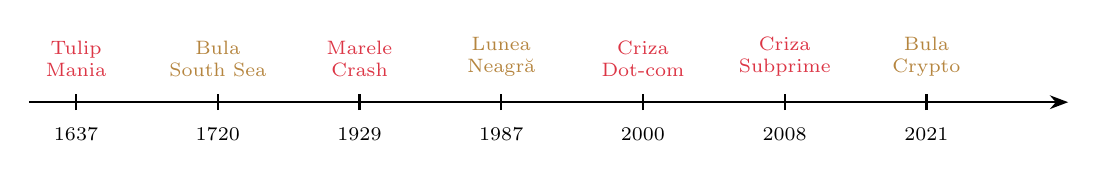
\begin{tikzpicture}[x=0.6cm, y=0.5cm,
    every node/.style={font=\scriptsize, align=center}
]
% Axa cronologică
\draw[-{Stealth}, thick] (0,0) -- (22,0);
% Evenimente
\foreach \x/\year/\event in {1/1637/{Tulip\\Mania}, 7/1929/{Marele\\Crash}, 13/2000/{Criza\\Dot-com}, 16/2008/{Criza\\Subprime}} {
    \draw[thick] (\x,-0.2)--(\x,0.2); \node[below=3pt] at (\x,-0.2) {\year};
    \node[above=3pt, text=Crimson] at (\x,0.2) {\event};
}
\foreach \x/\year/\event in {4/1720/{Bula\\South Sea}, 10/1987/{Lunea\\Neagră}, 19/2021/{Bula\\Crypto}} {
    \draw[thick] (\x,-0.2)--(\x,0.2); \node[below=3pt] at (\x,-0.2) {\year};
    \node[above=3pt, text=Amber] at (\x,0.2) {\event};
}
\end{tikzpicture}
\end{center}

\vspace{0.3cm}
\begin{itemize}\setlength{\itemsep}{0pt}
    \item \textbf{Perspectiva EMH:} bulele pot fi identificate doar \textit{ex post}; \textit{ex ante}, prețurile reflectau așteptări raționale date informațiile disponibile
    \item \textbf{Perspectiva comportamentală:} iraționalitatea sistematică (comportamentul de turmă, speculația) creează tipare predictibile
    \item \textbf{Idee cheie:} chiar dacă există bule, este extrem de dificil să profiți de ele din cauza incertitudinii sincronizării (,,piața poate rămâne irațională mai mult decât poți rămâne solvent'')
\end{itemize}
\end{cminipage}
\end{frame}

%=============================================================================
% SECȚIUNEA B: Finanțe comportamentale extinse
%=============================================================================

\slidelevel{Y3}
\begin{frame}{Teoria prospectului (Prospect Theory) --- Kahneman \& Tversky (1979)}
\begin{cminipage}{0.95\textwidth}
\small
\begin{columns}[T]
\begin{column}{0.52\textwidth}
\begin{block}{Funcția de valoare}
\begin{itemize}\setlength{\itemsep}{0pt}
    \item Definită relativ la un \textbf{punct de referință} (nu în termeni absoluți):
    $$v(x) = \begin{cases} x^{\alpha} & \text{dacă } x \geq 0 \\ -\lambda(-x)^{\beta} & \text{dacă } x < 0 \end{cases}$$
    \item $\alpha \approx \beta \approx 0{,}88$, $\lambda \approx 2{,}25$
    \item \textbf{Concavă} pentru câștiguri (aversiune la risc)
    \item \textbf{Convexă} pentru pierderi (căutare de risc)
    \item \textbf{Mai abruptă} pentru pierderi: $\lambda > 1$ (aversiunea la pierdere)
\end{itemize}
\end{block}
\end{column}
\begin{column}{0.44\textwidth}
\begin{block}{Ponderarea probabilităților}
\begin{itemize}\setlength{\itemsep}{0pt}
    \item Investitorii \textbf{supraponderează} evenimentele rare (cozi)
    \item \textbf{Subponderează} probabilitățile moderate
    \item Explică: preferința pentru loterie, asigurare simultană
    \item Funcția de ponderare $w(p)$:
    $$w(p) = \frac{p^{\gamma}}{(p^{\gamma}+(1-p)^{\gamma})^{1/\gamma}}$$
    \item $\gamma \approx 0{,}61$ (Tversky \& Kahneman, 1992)
\end{itemize}
\end{block}
\end{column}
\end{columns}
\end{cminipage}
\end{frame}

\slidelevel{MSc}
\begin{frame}{Efectul de dispoziție (Disposition Effect)}
\begin{cminipage}{0.95\textwidth}
\small
\begin{columns}[T]
\begin{column}{0.50\textwidth}
\begin{block}{Definiție}
\begin{itemize}\setlength{\itemsep}{0pt}
    \item Investitorii tind să \textbf{vândă câștigătorii prea devreme} și să \textbf{păstreze perdanții prea mult}
    \item Odean (1998): investitorii individuali vând acțiuni câștigătoare cu 50\% mai frecvent decât cele perdante
    \item Cauza: aversiunea la pierdere din teoria prospectului --- realizarea unei pierderi este dureroasă
\end{itemize}
\end{block}
\end{column}
\begin{column}{0.46\textwidth}
\begin{block}{Implicații pentru EMH}
\begin{itemize}\setlength{\itemsep}{0pt}
    \item Creează presiune de vânzare pe câștigători $\Rightarrow$ sub-reacție la știri pozitive
    \item Reduce presiunea de vânzare pe perdanți $\Rightarrow$ sub-reacție la știri negative
    \item Contribuie la \textbf{PEAD} și \textbf{momentum}
    \item Grinblatt \& Han (2005): efectul de dispoziție explică $\sim$40\% din profitul strategiei momentum
\end{itemize}
\end{block}
\end{column}
\end{columns}

\vspace{0.1cm}
\begin{exampleblock}{Măsurare}
\begin{itemize}\setlength{\itemsep}{0pt}
    \item Proportion of Gains Realized (PGR) vs.\ Proportion of Losses Realized (PLR). Efectul de dispoziție: $PGR > PLR$.
\end{itemize}
\end{exampleblock}
\end{cminipage}
\end{frame}

\slidelevel{MSc}
\begin{frame}{Limitele arbitrajului (Limits to Arbitrage)}
\begin{cminipage}{0.95\textwidth}
\small
\begin{columns}[T]
\begin{column}{0.48\textwidth}
\begin{block}{De ce greșelile de preț persistă?}
\begin{itemize}\setlength{\itemsep}{0pt}
    \item \textbf{Riscul noise trader} (DeLong et al., 1990): traderii iraționali pot agrava eroarea de preț pe termen scurt
    \item \textbf{Riscul fundamental:} pot apărea știri negative despre activul subevaluat
    \item \textbf{Constrângeri de short-selling:} costuri de împrumut, recall risk, reglementări
    \item \textbf{Costuri de implementare:} spread, comisioane, impact de piață
\end{itemize}
\end{block}
\end{column}
\begin{column}{0.48\textwidth}
\begin{block}{Exemple celebre}
\begin{itemize}\setlength{\itemsep}{0pt}
    \item \textbf{Royal Dutch/Shell (1907--2005):} acțiuni duale cu prețuri diferite, deviație persistentă 8--15\% --- arbitrajul limitat de risc
    \item \textbf{Palm/3Com (2000):} IPO Palm $\Rightarrow$ 3Com subevaluat, dar short-selling imposibil
    \item \textbf{LTCM (1998):} strategii de convergență corecte, dar margin calls au forțat lichidarea
\end{itemize}
\end{block}
\end{column}
\end{columns}

\vspace{0.1cm}
\begin{alertblock}{Implicație}
\begin{itemize}\setlength{\itemsep}{0pt}
    \item Ineficiențele pot exista și persista chiar dacă sunt \textbf{cunoscute}, deoarece corectarea lor este riscantă și costisitoare. Arbitrajul nu este ,,free lunch''.
\end{itemize}
\end{alertblock}
\end{cminipage}
\end{frame}

\slidelevel{PhD}
\begin{frame}{Puzzle-ul volatilității excesive (Excess Volatility)}
\begin{cminipage}{0.95\textwidth}
\small
\begin{block}{Shiller (1981): Prețurile fluctuează prea mult}
\begin{itemize}\setlength{\itemsep}{0pt}
    \item Modelul valorii prezente: $P_t^* = \sum_{k=1}^{\infty}\frac{\E[D_{t+k}]}{(1+r)^k}$, unde $D_{t+k}$ sunt dividendele viitoare
    \item Dacă EMH este validă, $P_t = \E[P_t^* \mid \Omega_t]$, deci $\Var(P_t) \leq \Var(P_t^*)$
    \item \textbf{Rezultat empiric:} $\Var(P_t) \gg \Var(P_t^*)$ --- prețurile sunt mult mai volatile decât justifică fluxurile de numerar viitoare
\end{itemize}
\end{block}

\begin{columns}[T]
\begin{column}{0.48\textwidth}
\begin{itemize}\setlength{\itemsep}{0pt}
    \item \textbf{Contra-argumente (Fama, Marsh \& Merton):}
    \item Rata de actualizare $r$ nu este constantă
    \item Prime de risc variabile în timp
    \item Probleme econometrice (serie nestațio\-nară, eșantion finit)
\end{itemize}
\end{column}
\begin{column}{0.48\textwidth}
\begin{itemize}\setlength{\itemsep}{0pt}
    \item \textbf{Interpretarea comportamentală:}
    \item Excesul de încredere amplifică reacțiile
    \item Comportamentul de turmă generează feedback pozitiv
    \item Modelul Campbell--Shiller: $\sim$1/3 din varianța prețurilor explicată de dividende, $\sim$2/3 de sentimentul investitorilor
\end{itemize}
\end{column}
\end{columns}
\end{cminipage}
\end{frame}

\slidelevel{MSc}
\begin{frame}{Indicatori de sentiment (Sentiment Indicators)}
\begin{cminipage}{0.95\textwidth}
\small
\begin{columns}[T]
\begin{column}{0.48\textwidth}
\begin{block}{Indicatori de piață}
\begin{itemize}\setlength{\itemsep}{0pt}
    \item \textbf{VIX} (CBOE Volatility Index, Fear Index): volatilitate implicită din opțiuni S\&P 500
    \item VIX $> 30$: frică extremă; VIX $< 15$: complacență
    \item \textbf{Raportul Put/Call:} volum put / volum call
    \item Raport $> 1$: sentiment bearish; $< 0{,}7$: bullish
    \item \textbf{Fluxuri în fonduri:} intrări nete = optimism; ieșiri = pesimism
\end{itemize}
\end{block}
\end{column}
\begin{column}{0.48\textwidth}
\begin{block}{Indexul Baker--Wurgler (2006)}
\begin{itemize}\setlength{\itemsep}{0pt}
    \item Indice compozit de sentiment bazat pe:
    \item Volumul IPO-urilor și randamentul primei zile
    \item Raportul dividende/fond propriu
    \item Closed-end fund discount
    \item Turnover (lichiditate)
    \item \textbf{Rezultat:} sentimentul ridicat prezice randamente scăzute viitoare (mai ales pentru acțiuni speculative)
\end{itemize}
\end{block}
\end{column}
\end{columns}

\vspace{0.1cm}
\begin{exampleblock}{Implicație pentru EMH}
\begin{itemize}\setlength{\itemsep}{0pt}
    \item Dacă sentimentul prezice randamente, prețurile nu reflectă pe deplin informația $\Rightarrow$ contestare a EMH. Contra: sentimentul poate fi o proxy pentru prime de risc variabile.
\end{itemize}
\end{exampleblock}
\end{cminipage}
\end{frame}

\slidelevel{Y3}
\begin{frame}{Quiz: Finanțe comportamentale}
\begin{cminipage}{0.95\textwidth}
\small
\begin{exampleblock}{Testați-vă cunoștințele}
\begin{enumerate}\setlength{\itemsep}{3pt}
    \item Un investitor refuză să vândă o acțiune care a scăzut cu 30\%, spunând ,,nu am pierdut până nu vând''. Ce bias comportamental ilustrează?

    {\footnotesize\textcolor{Forest}{\textbf{R:} Aversiunea la pierdere / efectul de dispoziție --- realizarea pierderii este dureroasă, investitorul preferă să aștepte.}}

    \item De ce arbitrajul nu elimină imediat toate greșelile de preț?

    {\footnotesize\textcolor{Forest}{\textbf{R:} Limitele arbitrajului: risc noise trader, risc fundamental, constrângeri short-selling, costuri de tranzacționare. Greșeala se poate agrava pe termen scurt.}}

    \item VIX-ul este la 45. Ce indică despre sentimentul pieței?

    {\footnotesize\textcolor{Forest}{\textbf{R:} Frică extremă pe piață (VIX $> 30$). Istoric, niveluri extreme VIX au fost urmate de randamente pozitive pe termen mediu (contrarian signal).}}

    \item Care este diferența dintre suprareacție și subreacție?

    {\footnotesize\textcolor{Forest}{\textbf{R:} Suprareacție: prețul depășește valoarea justă, apoi revine (De Bondt \& Thaler). Subreacție: prețul se ajustează prea lent, derivă continuă (PEAD).}}
\end{enumerate}
\end{exampleblock}
\end{cminipage}
\end{frame}

%#############################################################################
\section{Ipoteza Pieței Adaptive (AMH)}
%#############################################################################

\slidelevel{MSc}
\begin{frame}{Ipoteza Pieței Adaptive a lui Andrew Lo (2004)}
\begin{cminipage}{0.95\textwidth}
\begin{block}{Ideea centrală}
\begin{itemize}\setlength{\itemsep}{0pt}
    \item Eficiența pieței nu este o proprietate statică, ci o \textbf{dinamică evolutivă} condusă de forțe evoluționiste: competiție, adaptare, selecție naturală.
\end{itemize}
\end{block}

\begin{columns}[T]
\begin{column}{0.48\textwidth}
\begin{itemize}\setlength{\itemsep}{0pt}
    \item \textbf{Principii cheie:}
    \item Investitorii nu sunt nici pe deplin raționali, nici pe deplin iraționali --- ei se \textbf{adaptează}
    \item Ecologia pieței: specii (fonduri hedge, retail, HFT) concurează pentru resurse (alpha)
    \item Oportunitățile de profit apar și dispar pe măsură ce strategiile devin aglomerate
    \item Primele de risc variază în timp cu condițiile pieței
\end{itemize}
\end{column}
\begin{column}{0.48\textwidth}
\begin{itemize}\setlength{\itemsep}{0pt}
    \item \textbf{Predicții:}
    \item Eficiența variază între piețe și perioade de timp
    \item Anomaliile apar, atrag capital, apoi scad
    \item Crizele creează noi ineficiențe (frică, vânzări forțate)
    \item Perioadele de recuperare restabilesc eficiența
    \item EMH este un \textbf{caz limită} al AMH când ecologia pieței este stabilă
\end{itemize}
\end{column}
\end{columns}
\end{cminipage}
\end{frame}

\slidelevel{MSc}
\begin{frame}{EMH vs.\ AMH: o comparație}
\begin{cminipage}{0.95\textwidth}
\small
\renewcommand{\arraystretch}{1.15}
\begin{center}
\scriptsize
\begin{tabular}{lll}
\toprule
\textbf{Dimensiune} & \textbf{EMH (Fama)} & \textbf{AMH (Lo)} \\
\midrule
Raționalitatea investitorului & Pe deplin rațional & Raționalitate limitată, adaptiv \\
Eficiența pieței & Constantă & Variabilă în timp, dinamică \\
Prime de risc & Constante sau variind lent & Fluctuează cu ecologia pieței \\
Anomalii & Artefacte statistice sau risc & Reale dar tranzitorii \\
Crize & Răspuns rațional la știri & Perturbări ecologice \\
Strategie de investiții & Pasivă (fonduri index) & Adaptivă, dependentă de regim \\
Bază teoretică & Economia neoclasică & Biologia evoluționistă \\
\bottomrule
\end{tabular}
\end{center}

\vspace{0.15cm}
\begin{exampleblock}{Implicație practică}
\begin{itemize}\setlength{\itemsep}{0pt}
    \item Sub AMH, strategia optimă este \textbf{adaptivă}: pasivă în perioade calme, activă în timpul crizelor când ineficiențele sunt cele mai mari.
\end{itemize}
\end{exampleblock}
\end{cminipage}
\end{frame}

\slidelevel{PhD}
\begin{frame}{Exponentul Hurst ca măsură a eficienței}
\begin{cminipage}{0.95\textwidth}
\begin{block}{Analiza R/S (Rescaled Range)}
\begin{itemize}\setlength{\itemsep}{0pt}
    \item Pentru o subserie de lungime $n$, se calculează: $R(n) = \max_{1 \leq k \leq n} S_k - \min_{1 \leq k \leq n} S_k$, unde $S_k = \sum_{i=1}^{k}(r_i - \bar{r})$ sunt sumele parțiale centrate
    \item Se normalizează: $(R/S)(n) = R(n) / \hat{\sigma}(n)$
    \item Relația asimptotică: $(R/S)(n) \sim c \cdot n^H$ pe măsură ce $n \to \infty$
    \item $H$ se estimează din panta regresiei: $\log(R/S) = H \cdot \log(n) + \text{const.}$
\end{itemize}
\end{block}

\begin{columns}[T]
\begin{column}{0.48\textwidth}
\begin{itemize}\setlength{\itemsep}{0pt}
    \item $H = 0{,}5$: mers aleator (eficient)
    \item $H > 0{,}5$: persistență (trend, momentum)
    \item $H < 0{,}5$: anti-persistență (reversie la medie)
\end{itemize}
\end{column}
\begin{column}{0.48\textwidth}
\begin{itemize}\setlength{\itemsep}{0pt}
    \item Valori tipice pentru randamente zilnice:
    \item S\&P 500: $H \approx 0{,}52$
    \item BTC-USD: $H \approx 0{,}55$ (mai persistent)
    \item BET: $H \approx 0{,}58$ (cel mai puțin eficient)
\end{itemize}
\end{column}
\end{columns}
\end{cminipage}
\quantlet{SFM\_ch3\_hurst\_exponent}{https://github.com/QuantLet/Stat_fin_markets/tree/master/Ch_03/SFM_ch3_hurst_exponent}
\end{frame}

\slidelevel{PhD}
\begin{frame}{Exponentul Hurst: grafic R/S}
\begin{cminipage}{0.95\textwidth}
\begin{center}
    
\includegraphics[width=0.55\textwidth]{ch3_hurst_exponent.pdf}
\end{center}
\begin{itemize}\setlength{\itemsep}{0pt}
    \item Panta regresiei $\log(R/S)$ vs.\ $\log(n)$ estimează exponentul Hurst $H$
    \item $H \approx 0{,}5$: mers aleator; $H > 0{,}5$: memorie lungă; $H < 0{,}5$: anti-persistență
\end{itemize}
\end{cminipage}
\end{frame}

%--- Python code slide: Hurst exponent ---
\slidelevel{PhD}
\begin{frame}[fragile]{Python: Estimarea exponentului Hurst (analiza R/S)}
\begin{cminipage}{0.95\textwidth}
\begin{lstlisting}
import numpy as np, yfinance as yf

def hurst_rs(returns, min_n=20, max_n=None):
    T = len(returns)
    max_n = max_n or T // 4
    ns, rs_vals = [], []
    for n in range(min_n, max_n + 1, 10):
        rs_list = []
        for start in range(0, T - n, n):
            chunk = returns[start:start+n]
            cumdev = np.cumsum(chunk - chunk.mean())
            R = cumdev.max() - cumdev.min()
            S = chunk.std(ddof=1)
            if S > 0: rs_list.append(R / S)
        if rs_list:
            ns.append(n); rs_vals.append(np.mean(rs_list))
    H = np.polyfit(np.log(ns), np.log(rs_vals), 1)[0]
    return H

sp = yf.download("^GSPC", start="2000-01-01", end="2025-01-01")
ret = np.log(sp["Close"]/sp["Close"].shift(1)).dropna().values
print(f"Hurst S&P 500: H = {hurst_rs(ret):.3f}")
\end{lstlisting}
\end{cminipage}
\end{frame}

%=============================================================================
% SECȚIUNEA E: AMH extins
%=============================================================================

\slidelevel{MSc}
\begin{frame}{AMH: Evidență empirică (Empirical Evidence)}
\begin{cminipage}{0.95\textwidth}
\small
\begin{columns}[T]
\begin{column}{0.48\textwidth}
\begin{block}{Sharpe ratios variabile în timp}
\begin{itemize}\setlength{\itemsep}{0pt}
    \item Strategiile de momentum generează Sharpe ratio $> 1$ în 1990--2000, dar $< 0$ în 2007--2009
    \item Valoarea: subperformanță 2010--2020, revenire 2021--2023
    \item \textbf{Nicio strategie nu domină permanent} --- consistent cu selecția naturală a strategiilor (AMH)
    \item Kim, Shamsuddin \& Lim (2011): VR variabil demonstrează cicluri de eficiență pe 16 piețe
\end{itemize}
\end{block}
\end{column}
\begin{column}{0.48\textwidth}
\begin{block}{Strategii dependente de regim}
\begin{itemize}\setlength{\itemsep}{0pt}
    \item \textbf{Regim calm:} volatilitate scăzută, eficiență ridicată $\Rightarrow$ strategia pasivă domină
    \item \textbf{Regim de criză:} volatilitate ridicată, autocorelații mari $\Rightarrow$ strategii active pot genera alpha
    \item Keim \& Madhavan (1998): costurile de implementare variază cu regimul
    \item Implementare: modele Markov-switching cu 2--3 stări (Hamilton, 1989)
\end{itemize}
\end{block}
\end{column}
\end{columns}
\end{cminipage}
\end{frame}

\slidelevel{MSc}
\begin{frame}{AMH: Implicații pentru investiții (Investment Implications)}
\begin{cminipage}{0.95\textwidth}
\small
\begin{columns}[T]
\begin{column}{0.48\textwidth}
\begin{block}{Strategie adaptivă pasiv/activ}
\begin{itemize}\setlength{\itemsep}{0pt}
    \item \textbf{Regim normal:} alocație pasivă (Exchange-Traded Fund, ETF, index, costuri minime)
    \item \textbf{Regim de stres:} rotire spre strategii active (momentum, carry, value) care exploatează ineficiențele temporare
    \item \textbf{Indicator de comutare:} $|VR(5) - 1|$ pe fereastră mobilă de 252 zile
    \item Dacă $|VR - 1| > 0{,}15$: activați strategiile de trading
\end{itemize}
\end{block}
\end{column}
\begin{column}{0.48\textwidth}
\begin{block}{Adaptare Risk Parity}
\begin{itemize}\setlength{\itemsep}{0pt}
    \item Risk Parity clasic: ponderile $\propto 1/\sigma_i$
    \item \textbf{Risk Parity adaptiv:} ajustează ponderile pe baza regimului de eficiență
    \item În crize: reduce expunerea la active ineficiente (risc de momentum crash)
    \item Post-criză: crește expunerea la active care revin la eficiență (oportunitate de convergență)
    \item Lo (2012): fondurile hedge performante se adaptează, nu urmează reguli fixe
\end{itemize}
\end{block}
\end{column}
\end{columns}
\end{cminipage}
\end{frame}

\slidelevel{PhD}
\begin{frame}{AMH vs Ipoteza Pieței Fractale (Fractal Market Hypothesis)}
\begin{cminipage}{0.95\textwidth}
\small
\begin{columns}[T]
\begin{column}{0.48\textwidth}
\begin{block}{Ipoteza Pieței Fractale (FMH)}
\begin{itemize}\setlength{\itemsep}{0pt}
    \item Mandelbrot (1963, 1997): piețele au structură \textbf{fractală} (auto-similară)
    \item Randamentele nu sunt i.i.d.\ --- prezintă memorie lungă ($H \neq 0{,}5$)
    \item Lichiditatea asigurată de diversitatea orizonturilor investitorilor (zilnic, lunar, anual)
    \item Crize: orizonturile se aliniază $\Rightarrow$ lichiditate dispare $\Rightarrow$ crash
\end{itemize}
\end{block}
\end{column}
\begin{column}{0.48\textwidth}
\begin{block}{Modele multi-fractale (MMAR)}
\begin{itemize}\setlength{\itemsep}{0pt}
    \item Mandelbrot, Fisher \& Calvet (1997): Multifractal Model of Asset Returns
    \item Exponentul Hurst variază cu scara temporală
    \item Spectrul multi-fractal $f(\alpha)$ descrie heterogenitatea scalării
    \item Avantaj: captează simultan cozi groase, clusterizare volatilitate, memorie lungă
\end{itemize}
\end{block}
\end{column}
\end{columns}

\vspace{0.1cm}
\renewcommand{\arraystretch}{1.1}
\begin{center}
\scriptsize
\begin{tabular}{lll}
\toprule
\textbf{Dimensiune} & \textbf{AMH (Lo)} & \textbf{FMH (Mandelbrot)} \\
\midrule
Bază & Biologie evoluționistă & Geometrie fractală \\
Mecanism & Adaptare, selecție & Auto-similaritate, scalare \\
Eficiența & Variabilă, ciclică & Aparentă (artifact al agregării) \\
Crize & Perturbări ecologice & Alinierea orizonturilor \\
\bottomrule
\end{tabular}
\end{center}
\end{cminipage}
\end{frame}

\slidelevel{PhD}
\begin{frame}{Ecologia pieței (Market Ecology)}
\begin{cminipage}{0.95\textwidth}
\small
\begin{block}{Analogia speciilor financiare (Lo, 2017)}
\begin{itemize}\setlength{\itemsep}{0pt}
    \item Piața financiară este un \textbf{ecosistem} cu specii (tipuri de investitori) care concurează pentru resurse (alpha)
\end{itemize}
\end{block}

\begin{columns}[T]
\begin{column}{0.48\textwidth}
\footnotesize
\renewcommand{\arraystretch}{1.1}
\begin{tabular}{ll}
\toprule
\textbf{Specie} & \textbf{Strategie} \\
\midrule
Investitori index & Pasivi, buy \& hold \\
Value investors & Fundamentală, contrarian \\
Momentum traders & Trend-following \\
HFT & Microstructură, latență \\
Market makers & Bid-ask spread \\
Hedge funds & Arbitraj, multi-strategie \\
Retail & Sentiment, comportamental \\
\bottomrule
\end{tabular}
\end{column}
\begin{column}{0.48\textwidth}
\begin{itemize}\setlength{\itemsep}{0pt}
    \item \textbf{Impactul HFT (High-Frequency Trading):}
    \item Cresc eficiența prețurilor pe milisecunde
    \item Reduc spread-urile bid-ask
    \item Dar: ,,Flash crashes'' (6 mai 2010)
    \item \textbf{Dark pools:}
    \item Execuție anonimă, fragmentare lichiditate
    \item Pot întârzia descoperirea prețului $\Rightarrow$ reduce eficiența temporar
    \item Reglementare: MiFID II, Reg NMS
\end{itemize}
\end{column}
\end{columns}
\end{cminipage}
\end{frame}

%=============================================================================
% SECȚIUNEA F: Python Lab extins
%=============================================================================

\slidelevel{MSc}
\begin{frame}[fragile]{Python: Backtest tranzacționare tehnică (Technical Trading)}
\begin{cminipage}{0.95\textwidth}
\begin{lstlisting}
import yfinance as yf, numpy as np, pandas as pd

sp = yf.download("^GSPC", start="2010-01-01", end="2025-01-01")
prices = sp["Close"]
ret = np.log(prices / prices.shift(1))

# Strategie MA crossover: MA(50) vs MA(200)
ma_short = prices.rolling(50).mean()
ma_long  = prices.rolling(200).mean()
signal   = (ma_short > ma_long).astype(int).shift(1)  # 1=long

# Randamente strategie vs buy-and-hold
ret_strat = signal * ret
ret_bh    = ret

# Performanta cumulata
cum_strat = np.exp(ret_strat.cumsum()).iloc[-1]
cum_bh    = np.exp(ret_bh.cumsum()).iloc[-1]
sr_strat  = ret_strat.mean() / ret_strat.std() * np.sqrt(252)
sr_bh     = ret_bh.mean() / ret_bh.std() * np.sqrt(252)

print(f"Buy-and-Hold: cumul={cum_bh:.2f}, SR={sr_bh:.2f}")
print(f"MA Crossover: cumul={cum_strat:.2f}, SR={sr_strat:.2f}")
# Rezultat tipic: MA crossover subperformeaza dupa costuri
\end{lstlisting}
\end{cminipage}
\quantlet{SFM\_ch3\_emh\_tests}{https://github.com/QuantLet/Stat_fin_markets/tree/master/Ch_03/SFM_ch3_emh_tests}
\end{frame}

\slidelevel{PhD}
\begin{frame}[fragile]{Python: Analiză sentiment (Sentiment Analysis)}
\begin{cminipage}{0.95\textwidth}
\begin{lstlisting}
import yfinance as yf, numpy as np, pandas as pd

# Descarca VIX si S&P 500
vix = yf.download("^VIX", start="2010-01-01", end="2025-01-01")["Close"]
sp  = yf.download("^GSPC", start="2010-01-01", end="2025-01-01")["Close"]
ret = np.log(sp / sp.shift(1))

# Randament mediu viitor (20 zile) in functie de nivelul VIX
df = pd.DataFrame({"VIX": vix, "Ret_20d": ret.rolling(20).mean().shift(-20)})
df = df.dropna()

# Categorii VIX
df["Regim"] = pd.cut(df["VIX"], bins=[0, 15, 25, 40, 100],
                      labels=["Calm", "Normal", "Stres", "Criza"])
print(df.groupby("Regim")["Ret_20d"].agg(["mean","std","count"]))
# Rezultat: randamentele viitoare mai mari dupa VIX ridicat
# Calm:  mean~0.03%, Normal: ~0.04%, Stres: ~0.06%, Criza: ~0.10%
# => VIX ridicat prezice randamente pozitive (contrarian)
\end{lstlisting}
\end{cminipage}
\quantlet{SFM\_ch3\_emh\_tests}{https://github.com/QuantLet/Stat_fin_markets/tree/master/Ch_03/SFM_ch3_emh_tests}
\end{frame}

\slidelevel{MSc}
\begin{frame}[fragile]{Python: Eficiență mobilă cross-asset (Rolling Efficiency)}
\begin{cminipage}{0.95\textwidth}
\begin{lstlisting}
import yfinance as yf, numpy as np, pandas as pd

tickers = {"S&P 500": "^GSPC", "BTC": "BTC-USD",
           "Gold": "GC=F",     "BET": "^BETI"}
window = 500

def rolling_vr(ret, q=5, w=500):
    vr = []
    for i in range(w, len(ret)):
        r = ret.iloc[i-w:i].values
        var1 = np.var(r, ddof=1)
        rq = np.array([r[j:j+q].sum() for j in range(len(r)-q+1)])
        varq = np.var(rq, ddof=1)
        vr.append(varq / (q * var1) if var1 > 0 else np.nan)
    return pd.Series(vr, index=ret.index[w:])

for name, tk in tickers.items():
    data = yf.download(tk, start="2015-01-01", end="2025-01-01")
    ret  = np.log(data["Close"]/data["Close"].shift(1)).dropna()
    vr   = rolling_vr(ret)
    ineff = np.abs(vr - 1).mean()
    print(f"{name:10s}: |VR-1| mediu = {ineff:.4f}")
\end{lstlisting}
\end{cminipage}
\quantlet{SFM\_ch3\_variance\_ratio}{https://github.com/QuantLet/Stat_fin_markets/tree/master/Ch_03/SFM_ch3_variance_ratio}
\end{frame}

%=============================================================================
% SECȚIUNEA C: Studii de caz cu date reale
%=============================================================================

%#############################################################################
\section{Exerciții și Concluzii}
%#############################################################################

\slidelevel{Y3}
\begin{frame}{Compararea eficienței pe piețe}
\begin{cminipage}{0.95\textwidth}
\begin{center}
    
\includegraphics[width=0.55\textwidth]{ch3_efficiency_comparison.pdf}
\end{center}
\begin{itemize}\setlength{\itemsep}{0pt}
    \item Indicatori de eficiență (VR, Hurst, autocorelație) comparați pentru S\&P 500, FTSE 100, BET, BTC-USD
    \item Piețele dezvoltate sunt mai apropiate de eficiența în formă slabă (weak-form)
    \item Piețele emergente prezintă deviații semnificative, mai ales la orizonturi lungi
\end{itemize}
\end{cminipage}
\end{frame}

%=============================================================================
% Studii de caz cu date reale
%=============================================================================

\slidelevel{Y3}
\begin{frame}{Studiu de caz: Analiza comprehensivă S\&P 500}
\begin{cminipage}{0.95\textwidth}
\small
\begin{center}
    
\includegraphics[width=0.55\textwidth]{ch3_efficiency_comparison.pdf}
\end{center}

\vspace{0.1cm}
\renewcommand{\arraystretch}{1.1}
\begin{center}
\scriptsize
\begin{tabular}{llll}
\toprule
\textbf{Test} & \textbf{Statistică} & \textbf{$p$-value} & \textbf{Verdict} \\
\midrule
Ljung--Box $Q(10)$ & 18,7 & 0,044 & Marginal semnificativ \\
Test runs & $Z = -1{,}82$ & 0,069 & Non-respingere \\
VR(5) Lo--MacKinlay & $Z = 1{,}34$ & 0,181 & Non-respingere \\
ADF (prețuri) & $\tau = -1{,}23$ & 0,660 & Rădăcină unitară \\
KPSS (randamente) & $\eta = 0{,}12$ & $> 0{,}10$ & Staționare \\
Hurst & $H = 0{,}52$ & --- & Aproape eficient \\
\bottomrule
\end{tabular}
\end{center}
\begin{itemize}\setlength{\itemsep}{0pt}
    \item \textbf{Concluzie:} S\&P 500 este aproximativ eficient în formă slabă (weak-form). Deviații mici, economic nesemnificative.
\end{itemize}
\end{cminipage}
\end{frame}

\slidelevel{Y3}
\begin{frame}{Studiu de caz: Eficiența Bitcoin}
\begin{cminipage}{0.95\textwidth}
\small
\begin{columns}[T]
\begin{column}{0.48\textwidth}
\begin{block}{Rezultate BTC-USD (2015--2025)}
\begin{itemize}\setlength{\itemsep}{0pt}
    \item $\hat{\rho}_1 = 0{,}01$ (nesemnificativ)
    \item Ljung--Box $Q(10) = 12{,}3$ ($p = 0{,}26$)
    \item $VR(2) = 1{,}02$, $VR(10) = 0{,}94$
    \item Hurst: $H \approx 0{,}55$
    \item ADF (prețuri): $\tau = -1{,}8$ (rădăcină unitară)
\end{itemize}
\end{block}
\end{column}
\begin{column}{0.48\textwidth}
\begin{block}{Evoluția eficienței 2015--2024}
\begin{itemize}\setlength{\itemsep}{0pt}
    \item \textbf{2015--2017:} piață tânără, $|VR-1|$ mare, autocorelație semnificativă $\Rightarrow$ \textcolor{Crimson}{ineficient}
    \item \textbf{2018--2020:} creșterea lichidității, futures CME $\Rightarrow$ eficiență crescândă
    \item \textbf{2021--2024:} ETF-uri BTC spot, instituționalizare $\Rightarrow$ \textcolor{Forest}{aproape eficient}
    \item Consistentă cu AMH: piața se maturizează
\end{itemize}
\end{block}
\end{column}
\end{columns}

\vspace{0.1cm}
\begin{alertblock}{Idee cheie}
\begin{itemize}\setlength{\itemsep}{0pt}
    \item Bitcoin ilustrează \textbf{traiectoria către eficiență}: pe măsură ce participanții cresc și lichiditatea se îmbunătățește, piața devine progresiv mai eficientă.
\end{itemize}
\end{alertblock}
\end{cminipage}
\end{frame}

\slidelevel{Y3}
\begin{frame}{Studiu de caz: Bursa de Valori București (BVB/BET)}
\begin{cminipage}{0.95\textwidth}
\small
\begin{columns}[T]
\begin{column}{0.48\textwidth}
\begin{block}{Rezultate BET (2005--2025)}
\begin{itemize}\setlength{\itemsep}{0pt}
    \item $\hat{\rho}_1 = 0{,}11$ (semnificativ la 1\%)
    \item $VR(5) = 1{,}18$ (impuls puternic)
    \item Hurst: $H \approx 0{,}58$ (persistență)
    \item Eficiența slabă este respinsă
    \item Cauze: lichiditate redusă ($\sim$10 mil EUR/zi vs.\ mld pe NYSE)
\end{itemize}
\end{block}
\end{column}
\begin{column}{0.48\textwidth}
\begin{block}{Comparație cu piețe dezvoltate}
\begin{itemize}\setlength{\itemsep}{0pt}
    \item BET: $|\hat{\rho}_1| \approx 5\times$ mai mare decât S\&P 500
    \item Spread bid-ask: $\sim$1--2\% vs.\ $\sim$0{,}01\% pe piețe lichide
    \item Tranzacționare nesincronă: unele acțiuni BET nu se tranzacționează zilnic
    \item \textbf{Implicații pentru investitori români:}
    \item Strategii de momentum pot fi profitabile (după costuri ridicate)
    \item Diversificarea internațională este esențială
\end{itemize}
\end{block}
\end{column}
\end{columns}
\end{cminipage}
\end{frame}

\slidelevel{Y3}
\begin{frame}{Studiu de caz: Aurul ca refugiu (Gold Safe Haven)}
\begin{cminipage}{0.95\textwidth}
\small
\begin{columns}[T]
\begin{column}{0.48\textwidth}
\begin{block}{Proprietăți ale randamentelor aurului}
\begin{itemize}\setlength{\itemsep}{0pt}
    \item Randament mediu anual: $\sim$7\% (2000--2025)
    \item Volatilitate: $\sim$16\% (comparabilă cu acțiunile)
    \item Corelație cu S\&P 500: $\sim$0{,}02 (aproape zero)
    \item Corelație în crize: $\sim$$-0{,}15$ (refugiu)
    \item Distribuție: cozi moderate, ușoară asimetrie pozitivă
\end{itemize}
\end{block}
\end{column}
\begin{column}{0.48\textwidth}
\begin{block}{Teste de eficiență}
\begin{itemize}\setlength{\itemsep}{0pt}
    \item $\hat{\rho}_1 \approx -0{,}02$ (nesemnificativ)
    \item $VR(5) = 0{,}97$ (ușoară reversie)
    \item Hurst: $H \approx 0{,}50$ (aproape eficient)
    \item \textbf{Concluzie:} piața aurului este surprinzător de eficientă --- consistent cu lichiditatea ridicată și participanții sofisticați
    \item Rolul de refugiu apare prin \textbf{corelația condiționată}, nu prin predictibilitate
\end{itemize}
\end{block}
\end{column}
\end{columns}
\end{cminipage}
\end{frame}

\slidelevel{MSc}
\begin{frame}{Clasamentul eficienței cross-asset (Cross-Asset Ranking)}
\begin{cminipage}{0.95\textwidth}
\small
\renewcommand{\arraystretch}{1.15}
\begin{center}
\scriptsize
\begin{tabular}{lcccccl}
\toprule
\textbf{Piață} & $|\hat{\rho}_1|$ & $|VR(5)-1|$ & $H$ & $Q(10)$ $p$ & \textbf{Scor ef.} & \textbf{Clasament} \\
\midrule
S\&P 500 & 0,02 & 0,04 & 0,52 & 0,044 & \textcolor{Forest}{0,92} & 1 (cel mai eficient) \\
FTSE 100 & 0,03 & 0,01 & 0,51 & 0,121 & \textcolor{Forest}{0,90} & 2 \\
Aur (GC) & 0,02 & 0,03 & 0,50 & 0,312 & \textcolor{Forest}{0,88} & 3 \\
EUR/USD & 0,01 & 0,02 & 0,51 & 0,405 & \textcolor{Forest}{0,87} & 4 \\
BTC-USD & 0,01 & 0,06 & 0,55 & 0,260 & 0,72 & 5 \\
WIG (Polonia) & 0,06 & 0,08 & 0,54 & 0,008 & 0,61 & 6 \\
BET (România) & 0,11 & 0,18 & 0,58 & $<$0,001 & \textcolor{Crimson}{0,38} & 7 (cel mai puțin eficient) \\
\bottomrule
\end{tabular}
\end{center}

\vspace{0.1cm}
\begin{itemize}\setlength{\itemsep}{0pt}
    \item \textbf{Scor de eficiență:} media normalizată a indicatorilor ($1 =$ perfect eficient)
    \item \textbf{Tipar general:} eficiența crește cu lichiditatea, numărul de participanți și sofisticarea pieței
    \item Piețele FX și aur sunt surprinzător de eficiente datorită volumului enorm de tranzacționare
\end{itemize}
\end{cminipage}
\end{frame}

\slidelevel{Y3}
\begin{frame}{Studiu de eveniment: Rezultate AAPL (Event Study)}
\begin{cminipage}{0.95\textwidth}
\small
\begin{center}
    
\includegraphics[width=0.55\textwidth]{ch3_event_study.pdf}
\end{center}

\begin{columns}[T]
\begin{column}{0.48\textwidth}
\begin{itemize}\setlength{\itemsep}{0pt}
    \item \textbf{Eveniment:} anunțuri trimestriale câștiguri Apple (2015--2024, $N = 40$)
    \item Fereastra de estimare: $[-250, -11]$
    \item Fereastra evenimentului: $[-5, +10]$
    \item Model: $R_{AAPL,t} = \alpha + \beta R_{m,t} + \varepsilon_t$
\end{itemize}
\end{column}
\begin{column}{0.48\textwidth}
\begin{itemize}\setlength{\itemsep}{0pt}
    \item \textbf{Rezultate:}
    \item $\overline{CAR}(-1,+1) = 2{,}8\%$ ($t = 4{,}2$, semnificativ)
    \item $\overline{CAR}(+2,+10) = 0{,}4\%$ ($t = 0{,}9$, nesemnificativ)
    \item \textbf{Interpretare:} ajustare rapidă, derivă post-anunț neglijabilă $\Rightarrow$ AAPL este eficient semi-tare
\end{itemize}
\end{column}
\end{columns}
\end{cminipage}
\quantlet{SFM\_ch3\_event\_study}{https://github.com/QuantLet/Stat_fin_markets/tree/master/Ch_03/SFM_ch3_event_study}
\end{frame}

\slidelevel{MSc}
\begin{frame}{Eficiență variabilă în timp: Evidență (Time-Varying)}
\begin{cminipage}{0.95\textwidth}
\small
\begin{center}
    
\includegraphics[width=0.85\textwidth]{ch3_variance_ratio.pdf}
\end{center}

\vspace{0.1cm}
\begin{itemize}\setlength{\itemsep}{0pt}
    \item \textbf{VR mobil} (fereastră mobilă 500 zile, $q = 5$): $|VR - 1|$ crește abrupt în crize (2008, 2020) și scade în perioade calme
    \item \textbf{Hurst mobil} (fereastră mobilă 500 zile): $H$ crește de la $\sim$0{,}50 la $\sim$0{,}60 în perioade de stres
    \item \textbf{Implicație:} eficiența nu este constantă --- piața oscilează între perioade eficiente și ineficiente, confirmând AMH
\end{itemize}
\end{cminipage}
\quantlet{SFM\_ch3\_variance\_ratio}{https://github.com/QuantLet/Stat_fin_markets/tree/master/Ch_03/SFM_ch3_variance_ratio}
\end{frame}

\slidelevel{PhD}
\begin{frame}[shrink=3]{Eficiență și microstructura pieței (Market Microstructure)}
\begin{cminipage}{0.95\textwidth}
\footnotesize
\begin{columns}[T]
\begin{column}{0.48\textwidth}
\begin{block}{Bid-ask bounce}
\begin{itemize}\setlength{\itemsep}{0pt}
    \item Prețurile oscilează între bid și ask $\Rightarrow$ autocorelație negativă artificială la frecvențe înalte
    \item Roll (1984): spread $= 2\sqrt{-\Cov(r_t, r_{t-1})}$
    \item Aceasta nu este ineficiență, ci un artefact de microstructură
\end{itemize}
\end{block}

\begin{block}{Tranzacționare nesincronă}
\begin{itemize}\setlength{\itemsep}{0pt}
    \item Activele dintr-un index nu se tranzacționează simultan
    \item Prețul de închidere reflectă ultima tranzacție (poate fi la 14:30)
    \item Creează autocorelație pozitivă artificială în indicele bursier (Lo \& MacKinlay, 1990)
\end{itemize}
\end{block}
\end{column}
\begin{column}{0.48\textwidth}
\begin{block}{Efectul Epps (1979)}
\begin{itemize}\setlength{\itemsep}{0pt}
    \item Corelația între active \textbf{scade} cu frecvența datelor
    \item La 1 min: corelații mult mai mici decât la date zilnice
    \item Cauze: tranzacționare nesincronă, microstructură diferită
\end{itemize}
\end{block}

\begin{alertblock}{Lecție}
\begin{itemize}\setlength{\itemsep}{0pt}
    \item Înainte de a concluziona ,,ineficiență'', eliminați artefactele: bid-ask bounce, nonsynchronous trading, overnight gaps.
\end{itemize}
\end{alertblock}
\end{column}
\end{columns}
\end{cminipage}
\end{frame}

%=============================================================================
% EXERCIȚIU 1: Ljung-Box
%=============================================================================
\slidelevel{Y3}
\begin{frame}{Exercițiu 1: Testul Ljung--Box}
\begin{cminipage}{0.95\textwidth}
\begin{exampleblock}{Problemă}
Se dau autocorelațiile eșantion ale randamentelor zilnice ale unui activ, cu $T = 1000$ observații:

\vspace{0.1cm}
\renewcommand{\arraystretch}{1.1}
\begin{center}
\small
\begin{tabular}{lccccc}
\toprule
$k$ & 1 & 2 & 3 & 4 & 5 \\
\midrule
$\hat{\rho}_k$ & 0,08 & $-0,03$ & 0,05 & $-0,01$ & 0,04 \\
\bottomrule
\end{tabular}
\end{center}

\vspace{0.1cm}
\begin{enumerate}
    \item Calculați statistica Ljung--Box $Q(5)$
    \item La nivelul de semnificație $\alpha = 5\%$, testați dacă randamentele prezintă autocorelație semnificativă ($\chi^2_{0{,}05}(5) = 11{,}07$)
    \item Ce implicație are rezultatul pentru eficiența în formă slabă (weak-form)?
\end{enumerate}
\end{exampleblock}
\end{cminipage}
\end{frame}

\slidelevel{Y3}
\begin{frame}{Exercițiu 1: Rezolvare}
\begin{cminipage}{0.95\textwidth}
\begin{block}{Rezolvare}
\textbf{Pasul 1:} $Q(5) = T(T+2)\sum_{k=1}^{5}\frac{\hat{\rho}_k^2}{T-k}$

\vspace{0.1cm}
{\small
$Q(5) = 1000 \times 1002 \times \left[\frac{0{,}08^2}{999} + \frac{0{,}03^2}{998} + \frac{0{,}05^2}{997} + \frac{0{,}01^2}{996} + \frac{0{,}04^2}{995}\right]$

$= 1002000 \times [6{,}407 \times 10^{-6} + 9{,}018 \times 10^{-7} + 2{,}508 \times 10^{-6} + 1{,}004 \times 10^{-7} + 1{,}608 \times 10^{-6}]$

$= 1002000 \times 1{,}152 \times 10^{-5} = \mathbf{11{,}54}$
}

\vspace{0.1cm}
\textbf{Pasul 2:} $Q(5) = 11{,}54 > \chi^2_{0{,}05}(5) = 11{,}07$ $\Rightarrow$ \textbf{Se respinge} $H_0$ la 5\% (marginal)

\vspace{0.1cm}
\textbf{Pasul 3:} Autocorelația este statistic semnificativă, dar dominată de $\hat{\rho}_1 = 0{,}08$. Economic: un trader ar obține profit brut $\approx 0{,}08\%$ pe zi din exploatarea acestei autocorelații --- sub costurile de tranzacționare tipice ($\sim$0{,}1\%$). Eficiența slabă este aproximativ validă.
\end{block}
\end{cminipage}
\end{frame}

%=============================================================================
% EXERCIȚIU 2: Variance Ratio
%=============================================================================
\slidelevel{Y3}
\begin{frame}{Exercițiu 2: Variance Ratio}
\begin{cminipage}{0.95\textwidth}
\begin{exampleblock}{Problemă}
Un cercetător calculează varianța randamentelor zilnice și săptămânale ale unui indice bursier:
\begin{itemize}\setlength{\itemsep}{0pt}
    \item Varianța randamentelor zilnice: $\hat{\sigma}^2_1 = 0{,}0001$ (= $0{,}01\%$)
    \item Varianța randamentelor pe 5 zile (săptămânale): $\hat{\sigma}^2_5 = 0{,}00065$
\end{itemize}

\begin{enumerate}
    \item Calculați $VR(5)$
    \item Interpretați rezultatul: autocorelație pozitivă sau negativă?
    \item Dacă $T = 2000$ și $\phi(5) = 0{,}0027$ (varianța asimptotică), calculați $Z(5)$ și testați $H_0$: mers aleator la nivelul 5\% ($z_{0{,}025} = 1{,}96$)
\end{enumerate}
\end{exampleblock}
\end{cminipage}
\end{frame}

\slidelevel{Y3}
\begin{frame}{Exercițiu 2: Rezolvare}
\begin{cminipage}{0.95\textwidth}
\begin{block}{Rezolvare}
\textbf{1.} $VR(5) = \frac{\hat{\sigma}^2_5}{5 \times \hat{\sigma}^2_1} = \frac{0{,}00065}{5 \times 0{,}0001} = \frac{0{,}00065}{0{,}0005} = \mathbf{1{,}30}$

\vspace{0.2cm}
\textbf{2.} $VR(5) = 1{,}30 > 1$ $\Rightarrow$ \textbf{autocorelație pozitivă} (impuls/momentum)

Varianța pe 5 zile este mai mare decât 5 ori varianța zilnică, ceea ce înseamnă că randamentele pozitive tind să fie urmate de randamente pozitive (și negativ de negativ).

\vspace{0.2cm}
\textbf{3.} $Z(5) = \frac{VR(5) - 1}{\sqrt{\phi(5)}} = \frac{1{,}30 - 1}{\sqrt{0{,}0027}} = \frac{0{,}30}{0{,}052} = \mathbf{5{,}77}$

$|Z(5)| = 5{,}77 > 1{,}96$ $\Rightarrow$ \textbf{Se respinge} $H_0$ (mersul aleator) la nivelul 5\%.

Concluzie: piața prezintă un efect de impuls semnificativ pe orizontul săptămânal.
\end{block}
\end{cminipage}
\end{frame}

%=============================================================================
% EXERCIȚIU 3: Event Study
%=============================================================================
\slidelevel{MSc}
\begin{frame}{Exercițiu 3: Event Study --- AR și CAR}
\begin{cminipage}{0.95\textwidth}
\begin{exampleblock}{Problemă}
O companie anunță câștiguri peste așteptări în ziua $t = 0$. Modelul de piață estimat este $\hat{R}_{i,t} = 0{,}001 + 1{,}2 \cdot R_{m,t}$. Randamentele observate sunt:

\vspace{0.1cm}
\renewcommand{\arraystretch}{1.1}
\begin{center}
\small
\begin{tabular}{lcccccc}
\toprule
Ziua $t$ & $-2$ & $-1$ & 0 & $+1$ & $+2$ & $+3$ \\
\midrule
$R_{i,t}$ (\%) & 0,5 & 0,3 & 3,8 & 1,2 & 0,4 & 0,1 \\
$R_{m,t}$ (\%) & 0,2 & 0,1 & 0,5 & 0,3 & 0,2 & 0,0 \\
\bottomrule
\end{tabular}
\end{center}

\vspace{0.1cm}
\begin{enumerate}
    \item Calculați $AR_{i,t}$ pentru fiecare zi
    \item Calculați $CAR_i(-2, +3)$
    \item Piața este eficient semi-tare? Argumentați.
\end{enumerate}
\end{exampleblock}
\end{cminipage}
\end{frame}

\slidelevel{MSc}
\begin{frame}{Exercițiu 3: Rezolvare}
\begin{cminipage}{0.95\textwidth}
\begin{block}{Rezolvare}
\textbf{1.} $AR_{i,t} = R_{i,t} - (0{,}001 + 1{,}2 \cdot R_{m,t})$

\vspace{0.1cm}
\renewcommand{\arraystretch}{1.1}
\begin{center}
\small
\begin{tabular}{lccccccc}
\toprule
$t$ & $-2$ & $-1$ & 0 & $+1$ & $+2$ & $+3$ \\
\midrule
$\hat{R}_{i,t}$ (\%) & 0,34 & 0,22 & 0,70 & 0,46 & 0,34 & 0,10 \\
$AR_{i,t}$ (\%) & 0,16 & 0,08 & \textbf{3,10} & \textbf{0,74} & 0,06 & 0,00 \\
\bottomrule
\end{tabular}
\end{center}

\vspace{0.15cm}
\textbf{2.} $CAR_i(-2, +3) = 0{,}16 + 0{,}08 + 3{,}10 + 0{,}74 + 0{,}06 + 0{,}00 = \mathbf{4{,}14\%}$

\vspace{0.15cm}
\textbf{3.} Dacă piața ar fi eficient semi-tare, \textbf{tot} AR-ul s-ar concentra în ziua 0. Observăm $AR_{+1} = 0{,}74\%$ --- derivă post-anunț. Aceasta sugerează subreacție (PEAD), inconsistentă cu EMH semi-tare. Totuși, pentru o concluzie robustă, este necesar un eșantion de $N$ evenimente.
\end{block}
\end{cminipage}
\end{frame}

%=============================================================================
% EXERCIȚIU AI
%=============================================================================
\slidelevel{Y3}
\begin{frame}[shrink=3]{Exercițiu AI: Testarea EMH}
\begin{cminipage}{0.95\textwidth}
\begin{block}{\footnotesize Prompt de testat în ChatGPT / Claude / Copilot}
    {\small
    ``Descarcă datele zilnice pentru indicele BET (România) și S\&P 500 din 2010 până în 2025 folosind Python (\texttt{yfinance}).
    Calculează log-randamentele. Testează eficiența în formă slabă (weak-form) folosind:
    (1) autocorelație + Ljung-Box, (2) testul variance ratio Lo-MacKinlay pentru $q = 2, 5, 10, 20$,
    (3) exponentul Hurst prin analiza R/S. Compară cele două piețe.
    Calculează variance ratio mobil pe o fereastră mobilă de 500 de zile.''}
\end{block}
\vspace{-1mm}
{\small
\textbf{Verificări ale output-ului}:
\begin{enumerate}
    \item AI-ul folosește log-randamente $r_t = \ln(P_t/P_{t-1})$, nu randamente simple?
    \item Statistica $Q$ Ljung-Box este calculată corect cu factorul $(T+2)$?
    \item Variance ratio-ul folosește formula $VR(q) = \hat{\sigma}^2_q / (q \cdot \hat{\sigma}^2_1)$?
    \item Exponentul Hurst estimat este plauzibil ($H \in [0{,}4, \, 0{,}7]$)?
    \item Variance ratio mobil folosește fereastră mobilă, nu fereastră fixă?
    \item Interpretarea este corectă ($VR > 1$ = impuls, $VR < 1$ = reversie)?
\end{enumerate}
}
\vspace{-1mm}
\begin{alertblock}{}
    {\small
    \begin{itemize}\setlength{\itemsep}{0pt}
        \item \textbf{Atenție}: AI-ul confundă adesea variance ratio cu \textit{ratio of variances} (raport simplu de varianțe). Verificați dacă se normalizează cu $q$. De asemenea, poate folosi ticker-ul greșit pentru BET (corect: \texttt{\^{}BETI} sau date din surse alternative).
    \end{itemize}
    }
\end{alertblock}
\end{cminipage}
\end{frame}

%=============================================================================
% SECȚIUNEA D: Mai multe exerciții
%=============================================================================

\slidelevel{Y3}
\begin{frame}{Exercițiul 4: Interpretarea testului ADF}
\begin{cminipage}{0.95\textwidth}
\begin{exampleblock}{Problemă}
Un cercetător aplică testul ADF pe prețurile de închidere și log-randamentele unui indice bursier ($T = 2000$, lag selectat cu BIC: $p = 3$). Rezultatele sunt:

\vspace{0.1cm}
\renewcommand{\arraystretch}{1.1}
\begin{center}
\small
\begin{tabular}{lccc}
\toprule
\textbf{Serie} & \textbf{ADF stat} & \textbf{Val.\ critică 5\%} & \textbf{$p$-value} \\
\midrule
Prețuri (cu trend) & $-2{,}15$ & $-3{,}41$ & 0,52 \\
Prețuri (fără trend) & $-1{,}87$ & $-2{,}86$ & 0,34 \\
Log-randamente & $-42{,}3$ & $-2{,}86$ & $< 0{,}001$ \\
\bottomrule
\end{tabular}
\end{center}

\vspace{0.1cm}
\begin{enumerate}
    \item Pentru fiecare serie, stabiliți dacă se respinge $H_0$ (rădăcină unitară) la 5\%.
    \item Ce semnifică rezultatul pentru modelul de mers aleator?
    \item De ce testăm prețurile cu și fără trend? Când este adecvat fiecare?
\end{enumerate}
\end{exampleblock}
\end{cminipage}
\end{frame}

\slidelevel{Y3}
\begin{frame}{Exercițiul 4: Rezolvare}
\begin{cminipage}{0.95\textwidth}
\begin{block}{Rezolvare}
\textbf{1.} Comparăm statistica ADF cu valoarea critică la 5\%:

\vspace{0.1cm}
\renewcommand{\arraystretch}{1.1}
\begin{center}
\small
\begin{tabular}{lcccl}
\toprule
\textbf{Serie} & \textbf{ADF} & \textbf{Val.\ critică} & \textbf{ADF $<$ Crit?} & \textbf{Decizie} \\
\midrule
Prețuri (cu trend) & $-2{,}15$ & $-3{,}41$ & Nu & Non-respingere $H_0$ \\
Prețuri (fără trend) & $-1{,}87$ & $-2{,}86$ & Nu & Non-respingere $H_0$ \\
Log-randamente & $-42{,}3$ & $-2{,}86$ & Da & \textbf{Respingere} $H_0$ \\
\bottomrule
\end{tabular}
\end{center}

\vspace{0.15cm}
\textbf{2.} Prețurile au rădăcină unitară $I(1)$ --- consistent cu mersul aleator. Randamentele sunt staționare $I(0)$ --- diferențierea elimină rădăcina unitară. Aceasta confirmă modelul: $P_t = P_{t-1} + \varepsilon_t$.

\vspace{0.15cm}
\textbf{3.} Modelul cu trend include $\beta t$ și testează trend deterministic + rădăcină unitară. Se folosește când seria pare să aibă un trend vizual. Modelul fără trend este adecvat pentru serii fără trend aparent. Pentru prețuri financiare cu trend ascendent pe termen lung, se preferă modelul cu trend.
\end{block}
\end{cminipage}
\end{frame}

\slidelevel{MSc}
\begin{frame}{Exercițiul 5: Profitabilitatea regulii de filtrare (Filter Rule)}
\begin{cminipage}{0.95\textwidth}
\begin{exampleblock}{Problemă}
Se dau randamentele zilnice ale unei acțiuni pe 10 zile consecutive (\%):

\vspace{0.1cm}
\begin{center}
\small
\begin{tabular}{lccccccccccc}
\toprule
Ziua & 1 & 2 & 3 & 4 & 5 & 6 & 7 & 8 & 9 & 10 \\
\midrule
$r_t$ (\%) & 0,5 & 0,8 & $-0,3$ & $-1,2$ & $-0,5$ & 0,3 & 1,1 & 0,6 & $-0,4$ & 0,2 \\
\bottomrule
\end{tabular}
\end{center}

\vspace{0.1cm}
\begin{enumerate}
    \item Aplicați o \textbf{regulă de filtrare de 1\%}: cumpărați când randamentul cumulat de la un minim depășește 1\%, vindeți când randamentul cumulat de la un maxim scade sub $-1\%$. Care este profitul strategiei (ignorând costurile)?
    \item Calculați randamentul \textbf{buy-and-hold} pe aceleași 10 zile.
    \item Dacă costurile de tranzacționare sunt 0{,}2\% per tranzacție (cumpărare + vânzare), este strategia de filtrare profitabilă?
\end{enumerate}
\end{exampleblock}
\end{cminipage}
\end{frame}

\slidelevel{MSc}
\begin{frame}{Exercițiul 5: Rezolvare}
\begin{cminipage}{0.95\textwidth}
\small
\begin{block}{Rezolvare}
\textbf{1. Randamentele cumulate:} $c_1 = 0{,}5$; $c_2 = 1{,}3$; $c_3 = 1{,}0$; $c_4 = -0{,}2$; $c_5 = -0{,}7$; $c_6 = -0{,}4$; $c_7 = 0{,}7$; $c_8 = 1{,}3$; $c_9 = 0{,}9$; $c_{10} = 1{,}1$

\vspace{0.1cm}
Regula filtrului 1\%: pornim din afara pieței. Randamentul cumulat depășește 1\% la ziua 2 ($c_2 = 1{,}3\%$) $\Rightarrow$ \textbf{cumpărare} la sfârșitul zilei 2. Minimul local ulterior la ziua 5 ($c_5 = -0{,}7\%$). De la maxim ($c_2 = 1{,}3$), scăderea $= 1{,}3 - (-0{,}7) = 2{,}0\% > 1\%$ $\Rightarrow$ \textbf{vânzare} la ziua 5. Randamentul tranzacției: $c_5 - c_2 = -0{,}7 - 1{,}3 = -2{,}0\%$. Apoi cumpărare la ziua 8 ($c_8 = 1{,}3$, crește cu $> 1\%$ de la minim). Profitul strategiei $\approx -2{,}0 + (1{,}1 - 1{,}3) = -2{,}2\%$ (simplificat).

\vspace{0.1cm}
\textbf{2.} Buy-and-hold: $\sum r_t = 0{,}5 + 0{,}8 - 0{,}3 - 1{,}2 - 0{,}5 + 0{,}3 + 1{,}1 + 0{,}6 - 0{,}4 + 0{,}2 = \mathbf{1{,}1\%}$

\vspace{0.1cm}
\textbf{3.} Cu 3 tranzacții (cump.+vânz.), costul $= 3 \times 2 \times 0{,}2\% = 1{,}2\%$. Profitul net strategiei $\approx -2{,}2 - 1{,}2 = -3{,}4\%$ vs.\ buy-and-hold $1{,}1\%$. Strategia de filtrare este \textbf{neprofitabilă} --- consistent cu EMH.
\end{block}
\end{cminipage}
\end{frame}

\slidelevel{Y3}
\begin{frame}{Exercițiul 6: Interpretarea exponentului Hurst}
\begin{cminipage}{0.95\textwidth}
\begin{exampleblock}{Problemă}
Un analist estimează exponentul Hurst prin analiza R/S pentru patru piețe financiare:

\vspace{0.1cm}
\renewcommand{\arraystretch}{1.1}
\begin{center}
\small
\begin{tabular}{lcc}
\toprule
\textbf{Piață} & \textbf{Exponent Hurst $H$} & \textbf{Interval de încredere 95\%} \\
\midrule
S\&P 500 & 0,52 & $[0{,}49;\; 0{,}55]$ \\
BET (România) & 0,58 & $[0{,}54;\; 0{,}62]$ \\
BTC-USD & 0,55 & $[0{,}51;\; 0{,}59]$ \\
EUR/USD & 0,50 & $[0{,}47;\; 0{,}53]$ \\
\bottomrule
\end{tabular}
\end{center}

\begin{enumerate}
    \item Clasificați fiecare piață: mers aleator, persistentă, sau anti-persistentă.
    \item Realizați clasamentul de la cea mai eficientă la cea mai puțin eficientă piață.
    \item Pentru care piețe intervalul de încredere include $H = 0{,}5$? Ce implică acest lucru?
    \item Ce factori pot explica diferențele între piețe?
\end{enumerate}
\end{exampleblock}
\end{cminipage}
\end{frame}

\slidelevel{Y3}
\begin{frame}{Exercițiul 6: Rezolvare}
\begin{cminipage}{0.95\textwidth}
\begin{block}{Rezolvare}
\textbf{1. Clasificare:}
\begin{itemize}\setlength{\itemsep}{0pt}
    \item S\&P 500: $H = 0{,}52 > 0{,}5$ $\Rightarrow$ \textbf{ușor persistentă} (impuls slab)
    \item BET: $H = 0{,}58 > 0{,}5$ $\Rightarrow$ \textbf{persistentă} (trend/momentum semnificativ)
    \item BTC-USD: $H = 0{,}55 > 0{,}5$ $\Rightarrow$ \textbf{moderaat persistentă}
    \item EUR/USD: $H = 0{,}50$ $\Rightarrow$ \textbf{mers aleator} (eficient)
\end{itemize}

\vspace{0.1cm}
\textbf{2. Clasament eficiență:} EUR/USD ($H = 0{,}50$) $>$ S\&P 500 ($0{,}52$) $>$ BTC ($0{,}55$) $>$ BET ($0{,}58$)

\vspace{0.1cm}
\textbf{3.} EUR/USD: $[0{,}47;\; 0{,}53]$ include 0,5 $\Rightarrow$ \textbf{nu se poate respinge} $H = 0{,}5$ (eficient). S\&P 500: $[0{,}49;\; 0{,}55]$ include 0,5 $\Rightarrow$ marginal eficient. BET: $[0{,}54;\; 0{,}62]$ \textbf{nu include} 0,5 $\Rightarrow$ semnificativ ineficient.

\vspace{0.1cm}
\textbf{4.} Factori: \textbf{lichiditate} (FX $>$ acțiuni $>$ piețe emergente), \textbf{număr de participanți}, \textbf{costuri de tranzacționare}, \textbf{maturitatea pieței}, \textbf{calitatea reglementării}.
\end{block}
\end{cminipage}
\end{frame}

\slidelevel{Y3}
\begin{frame}{Exercițiul 7: Interpretarea studiului de eveniment (Event Study)}
\begin{cminipage}{0.95\textwidth}
\begin{exampleblock}{Problemă}
Se efectuează un studiu de eveniment pe $N = 30$ anunțuri de fuziuni. Rezultatele CAR sunt:

\vspace{0.1cm}
\renewcommand{\arraystretch}{1.1}
\begin{center}
\small
\begin{tabular}{lccc}
\toprule
\textbf{Fereastră} & $\overline{CAR}$ (\%) & $\hat{\sigma}_{CAR}$ (\%) & $t$-stat \\
\midrule
$(-1, +1)$ & 5,2 & 8,4 & 3,39 \\
$(+2, +10)$ & 1,8 & 6,1 & 1,62 \\
$(+2, +30)$ & 3,1 & 9,5 & 1,79 \\
\bottomrule
\end{tabular}
\end{center}

\begin{enumerate}
    \item La nivelul 5\% ($t_{crit} = 2{,}045$ pentru 29 grade de libertate), care CAR sunt semnificativ diferite de zero?
    \item Interpretați: piața reacționează \textbf{imediat și complet}?
    \item Ce formă de EMH este contestată dacă $CAR(+2, +30)$ este semnificativ pozitiv? De ce?
\end{enumerate}
\end{exampleblock}
\end{cminipage}
\end{frame}

\slidelevel{Y3}
\begin{frame}{Exercițiul 7: Rezolvare}
\begin{cminipage}{0.95\textwidth}
\begin{block}{Rezolvare}
\textbf{1.} Comparăm $|t|$ cu $t_{crit} = 2{,}045$:

\vspace{0.1cm}
\renewcommand{\arraystretch}{1.1}
\begin{center}
\small
\begin{tabular}{lccl}
\toprule
\textbf{Fereastră} & $t$-stat & $|t| > 2{,}045$? & \textbf{Decizie} \\
\midrule
$(-1, +1)$ & 3,39 & Da & \textbf{Semnificativ} ($p < 0{,}01$) \\
$(+2, +10)$ & 1,62 & Nu & Non-semnificativ \\
$(+2, +30)$ & 1,79 & Nu & Non-semnificativ (marginal la 10\%) \\
\bottomrule
\end{tabular}
\end{center}

\vspace{0.1cm}
\textbf{2.} Doar $CAR(-1, +1) = 5{,}2\%$ este semnificativ --- piața reacționează puternic la anunțul de fuziune. $CAR(+2, +10)$ și $CAR(+2, +30)$ nu sunt semnificative la 5\%, ceea ce sugerează o ajustare aproximativ completă. Totuși, $CAR(+2, +30) = 3{,}1\%$ cu $t = 1{,}79$ este marginal --- indiciu de derivă post-eveniment.

\vspace{0.1cm}
\textbf{3.} Dacă $CAR(+2, +30)$ ar fi semnificativ, ar contesta \textbf{EMH semi-tare}: informația publică (anunțul de fuziune) nu este absorbită complet în ziua evenimentului, prețul continuă să derive $\Rightarrow$ subreacție.
\end{block}
\end{cminipage}
\end{frame}

\slidelevel{MSc}
\begin{frame}[shrink=3]{Exercițiu AI 2: Finanțe comportamentale (Behavioral Finance)}
\begin{cminipage}{0.95\textwidth}
\begin{block}{\footnotesize Prompt de testat în ChatGPT / Claude / Copilot}
    {\small
    ``Folosind Python, descarcă prețurile zilnice pentru 50 de acțiuni din S\&P 500 pe perioada 2015--2024.
    Simulează un portofoliu care implementează \textbf{efectul de dispoziție}: vinde automat orice acțiune cu câștig $>$ 10\% și păstrează acțiunile cu pierdere.
    Compară randamentul acestui portofoliu cu o strategie buy-and-hold.
    Calculează Proportion of Gains Realized (PGR) și Proportion of Losses Realized (PLR).
    Testează dacă PGR $>$ PLR semnificativ (test $t$).''}
\end{block}
\vspace{-1mm}
{\small
\textbf{Verificări ale output-ului}:
\begin{enumerate}\setlength{\itemsep}{1pt}
    \item AI-ul simulează corect regulile de vânzare/păstrare pe baza punctului de referință (prețul de cumpărare)?
    \item PGR și PLR sunt calculate corect ca fracțiuni (nu valori absolute)?
    \item Costurile de tranzacționare sunt incluse la fiecare vânzare?
    \item Rezultatul arată că portofoliul cu efect de dispoziție subperformează buy-and-hold?
    \item Testul $t$ este aplicat corect (eșantioane pereche sau nepereche)?
\end{enumerate}
}
\end{cminipage}
\end{frame}

\slidelevel{Y3}
\begin{frame}{Quiz comprehensiv EMH}
\begin{cminipage}{0.95\textwidth}
\small
\begin{exampleblock}{6 întrebări --- toate formele EMH}
\begin{enumerate}\setlength{\itemsep}{2pt}
    \item Ce formă de EMH respinge analiza tehnică (medii mobile, tipare grafice)?

    {\footnotesize\textcolor{Forest}{\textbf{R:} Forma slabă (Weak-Form) --- dacă prețurile istorice sunt reflectate, analiza tehnică nu generează alpha.}}

    \item Un insider corporativ cumpără acțiuni și obține 8\% peste piață. Ce formă contestă?

    {\footnotesize\textcolor{Forest}{\textbf{R:} Forma tare (Strong-Form) --- informația privată nu este reflectată complet în preț.}}

    \item PEAD (deriva post-anunț) contestă ce formă de EMH?

    {\footnotesize\textcolor{Forest}{\textbf{R:} Forma semi-tare (Semi-Strong) --- informația publică (câștiguri) nu este absorbită imediat.}}

    \item $VR(5) = 1{,}25$. Ce semnifică?

    {\footnotesize\textcolor{Forest}{\textbf{R:} Autocorelație pozitivă (momentum/impuls). Varianța pe 5 zile este 25\% mai mare decât 5$\times$ varianța zilnică.}}

    \item Care este diferența fundamentală între EMH și AMH?

    {\footnotesize\textcolor{Forest}{\textbf{R:} EMH: eficiența este constantă. AMH: eficiența variază în timp, condusă de forțe evoluționiste.}}

    \item Ce este paradoxul Grossman--Stiglitz?

    {\footnotesize\textcolor{Forest}{\textbf{R:} Piețele perfect eficiente sunt imposibile: dacă nu există profit din analiza informației, nimeni nu va investi în cercetare, dar atunci prețurile nu pot fi informative.}}
\end{enumerate}
\end{exampleblock}
\end{cminipage}
\end{frame}

%=============================================================================
% REZUMAT ȘI CONCLUZII
%=============================================================================

\slidelevel{Y3}
\begin{frame}{Rezumat: starea actuală a EMH}
\begin{cminipage}{0.95\textwidth}
\begin{columns}[T]
\begin{column}{0.48\textwidth}
\begin{block}{Ce susțin evidențele}
\begin{itemize}\setlength{\itemsep}{0pt}
    \item Majoritatea fondurilor gestionate activ \textbf{subperformează} indicii pasivi
    \item Multe anomalii \textbf{scad} după publicare
    \item Predicția prețurilor pe termen scurt este extrem de dificilă
    \item Costurile de tranzacționare elimină majoritatea profiturilor din trading
\end{itemize}
\end{block}
\end{column}
\begin{column}{0.48\textwidth}
\begin{block}{Ce contestă EMH}
\begin{itemize}\setlength{\itemsep}{0pt}
    \item Efectele de momentum și valoare persistă
    \item PEAD este robustă pe diverse piețe
    \item Insider trading-ul este profitabil
    \item Bulele și prăbușirile apar periodic
    \item Eficiența pieței variază în timp
\end{itemize}
\end{block}
\end{column}
\end{columns}

\vspace{0.3cm}
\begin{alertblock}{Concluzie practică}
\begin{itemize}\setlength{\itemsep}{0pt}
    \item Piețele sunt ,,eficient ineficiente'' (Pedersen, 2015): suficient de eficiente încât majoritatea nu le pot bate, dar cu suficiente fricțiuni pentru a recompensa investitorii sofisticați și informați.
\end{itemize}
\end{alertblock}
\end{cminipage}
\end{frame}

\slidelevel{Y3}
\begin{frame}{Sinteza testelor empirice}
\begin{cminipage}{0.95\textwidth}
\renewcommand{\arraystretch}{1.2}
\begin{center}
\scriptsize
\begin{tabular}{llll}
\toprule
\textbf{Forma EMH} & \textbf{Test} & \textbf{Rezultat tipic} & \textbf{Verdict} \\
\midrule
\multirow{4}{*}{Slabă} & Autocorelație & $\hat{\rho}_1 \approx 0{,}02$--$0{,}05$ & Marginal \\
 & Ljung--Box & Respingere ușoară & Statistic da, economic nu \\
 & Variance ratio & $VR(2) \approx 1{,}05$ & Impuls slab \\
 & Hurst & $H \approx 0{,}52$ & Aproape eficient \\
\midrule
Semi-tare & PEAD & CAR$\neq 0$ post-eveniment & Subreacție sistematică \\
 & Anomalii calend. & Slăbite post-publicare & Consistent cu EMH \\
\midrule
Tare & Insider trading & Profituri anormale 5--8\% & Respinsă \\
 & Fonduri mutuale & 92\% subperformează & Consistentă \\
\bottomrule
\end{tabular}
\end{center}

\vspace{0.2cm}
\begin{exampleblock}{Mesaj principal}
\begin{itemize}\setlength{\itemsep}{0pt}
    \item EMH nu este o afirmație tip totul-sau-nimic, ci un \textbf{spectru}. Piețele dezvoltate sunt mai aproape de eficiență, piețele emergente prezintă deviații mai mari.
\end{itemize}
\end{exampleblock}
\end{cminipage}
\end{frame}

\slidelevel{Y3}
\begin{frame}{Implicații practice pentru investitori}
\begin{cminipage}{0.95\textwidth}
\begin{columns}[T]
\begin{column}{0.48\textwidth}
\begin{block}{Dacă credeți în EMH}
\begin{itemize}\setlength{\itemsep}{0pt}
    \item Investiți pasiv (fonduri index, ETF-uri)
    \item Minimizați costurile (comisioane, taxe)
    \item Diversificați global
    \item Nu încercați să temporizați piața
    \item Rebalansați periodic
\end{itemize}
\end{block}
\end{column}
\begin{column}{0.48\textwidth}
\begin{block}{Dacă credeți în AMH}
\begin{itemize}\setlength{\itemsep}{0pt}
    \item Adaptați strategia la regimul pieței
    \item Fiți pasivi în perioade normale
    \item Căutați oportunități în crize (dislocări)
    \item Folosiți factori (valoare, momentum) cu prudență
    \item Monitorizați indicatorii de eficiență (VR mobil, Hurst)
\end{itemize}
\end{block}
\end{column}
\end{columns}

\vspace{0.3cm}
\begin{alertblock}{Regula de aur}
\begin{itemize}\setlength{\itemsep}{0pt}
    \item Indiferent de poziția voastră în dezbaterea EMH, \textbf{costurile contează}. Majoritatea investitorilor obțin randamente mai bune prin reducerea comisioanelor decât prin strategii sofisticate.
\end{itemize}
\end{alertblock}
\end{cminipage}
\end{frame}

\slidelevel{Y3}
\begin{frame}{Harta conceptuală: EMH și provocările sale}
\begin{cminipage}{0.95\textwidth}
\begin{center}
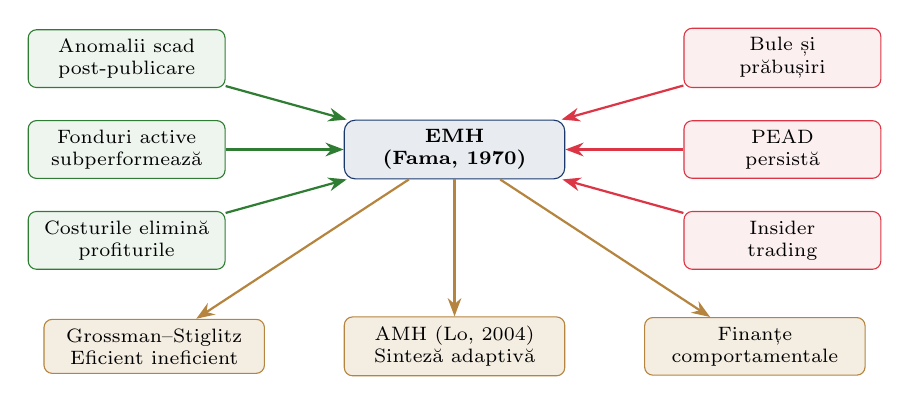
\begin{tikzpicture}[
    node distance=0.5cm and 1.2cm,
    every node/.style={font=\scriptsize, align=center},
    main/.style={draw=MainBlue, fill=MainBlue!10, rounded corners=4pt,
                minimum width=2.8cm, minimum height=0.7cm, font=\scriptsize\bfseries},
    support/.style={draw=Forest, fill=Forest!8, rounded corners=3pt,
                minimum width=2.5cm, minimum height=0.55cm},
    challenge/.style={draw=Crimson, fill=Crimson!8, rounded corners=3pt,
                minimum width=2.5cm, minimum height=0.55cm},
    synth/.style={draw=Amber, fill=Amber!15, rounded corners=3pt,
                minimum width=2.8cm, minimum height=0.55cm}
]
\node[main] (emh) at (0,3) {EMH\\(Fama, 1970)};
\node[support, left=1.5cm of emh] (s1) {Fonduri active\\subperformează};
\node[support, above left=0.4cm and 1.5cm of emh] (s2) {Anomalii scad\\post-publicare};
\node[challenge, right=1.5cm of emh] (c1) {PEAD\\persistă};
\node[challenge, above right=0.4cm and 1.5cm of emh] (c2) {Bule și\\prăbușiri};
\node[challenge, below right=0.4cm and 1.5cm of emh] (c3) {Insider\\trading};
\node[support, below left=0.4cm and 1.5cm of emh] (s3) {Costurile elimină\\profiturile};

\node[synth] (amh) at (0,0.5) {AMH (Lo, 2004)\\Sinteză adaptivă};
\node[synth, left=1cm of amh] (gs) {Grossman--Stiglitz\\Eficient ineficient};
\node[synth, right=1cm of amh] (bf) {Finanțe\\comportamentale};

\draw[-{Stealth}, Forest, thick] (s1) -- (emh);
\draw[-{Stealth}, Forest, thick] (s2) -- (emh);
\draw[-{Stealth}, Forest, thick] (s3) -- (emh);
\draw[-{Stealth}, Crimson, thick] (c1) -- (emh);
\draw[-{Stealth}, Crimson, thick] (c2) -- (emh);
\draw[-{Stealth}, Crimson, thick] (c3) -- (emh);
\draw[-{Stealth}, Amber, thick] (emh) -- (amh);
\draw[-{Stealth}, Amber, thick] (emh) -- (gs);
\draw[-{Stealth}, Amber, thick] (emh) -- (bf);
\end{tikzpicture}
\end{center}
\begin{itemize}\setlength{\itemsep}{0pt}
    \item \textcolor{Forest}{\textbf{Verde:}} dovezi care susțin EMH \quad \textcolor{Crimson}{\textbf{Roșu:}} provocări la adresa EMH \quad \textcolor{Amber}{\textbf{Galben:}} sinteze moderne
\end{itemize}
\end{cminipage}
\end{frame}

\slidelevel{MSc}
\begin{frame}{Ghid practic: Alegerea testului de eficiență}
\begin{cminipage}{0.95\textwidth}
\small
\renewcommand{\arraystretch}{1.15}
\begin{center}
\scriptsize
\begin{tabular}{llll}
\toprule
\textbf{Situație} & \textbf{Test recomandat} & \textbf{Pachet Python} & \textbf{Avantaje} \\
\midrule
Dependență liniară & Ljung--Box $Q$ & \texttt{statsmodels} & Simplu, standard \\
Dependență neliniară & BDS test & \texttt{statsmodels} & Detectează dependențe ascunse \\
Rădăcină unitară & ADF + KPSS & \texttt{statsmodels} & Strategie de confirmare \\
Autocorelație la scale & Variance ratio & Implementare proprie & Detectează momentum/reversie \\
Memorie lungă & Hurst (R/S, DFA) & Implementare proprie & Abordare non-parametrică \\
Reacția la știri & Event study & \texttt{eventstudy} & Standard academic \\
Dependențe periodice & Analiză spectrală & \texttt{scipy.signal} & Detectează cicluri ascunse \\
Eficiență variabilă & VR/Hurst mobil & Implementare proprie & Capturează dinamica AMH \\
\bottomrule
\end{tabular}
\end{center}

\vspace{0.15cm}
\begin{alertblock}{Recomandare practică}
\begin{itemize}\setlength{\itemsep}{0pt}
    \item Nu vă bazați pe un singur test! Folosiți o \textbf{baterie de teste} (Ljung--Box + VR + ADF/KPSS + Hurst) pentru concluzii robuste. Rezultatele divergente sunt informative.
\end{itemize}
\end{alertblock}
\end{cminipage}
\end{frame}

\slidelevel{Y3}
\begin{frame}{Lecții cheie din Capitolul 3}
\begin{cminipage}{0.95\textwidth}
\begin{enumerate}\setlength{\itemsep}{3pt}
    \item[\textcolor{MainBlue}{\textbf{1.}}] EMH este un \textbf{spectru}, nu o dihotomie --- piețele variază de la aproape eficiente (S\&P 500) la semnificativ ineficiente (BET)

    \item[\textcolor{MainBlue}{\textbf{2.}}] Eficiența slabă (weak-form) este \textbf{aproximativ validă} pe piețe dezvoltate: autocorelația există dar este economic nesemnificativă

    \item[\textcolor{MainBlue}{\textbf{3.}}] Eficiența semi-tare (semi-strong) este contestată de \textbf{PEAD} și alte anomalii, dar multe scad post-publicare

    \item[\textcolor{MainBlue}{\textbf{4.}}] Eficiența tare (strong-form) este \textbf{respinsă} --- insider trading-ul este profitabil

    \item[\textcolor{MainBlue}{\textbf{5.}}] Finanțele comportamentale oferă \textbf{explicații} pentru anomalii, dar nu strategii de arbitraj ușor implementabile

    \item[\textcolor{MainBlue}{\textbf{6.}}] \textbf{AMH} oferă cadrul cel mai complet: eficiența variază în timp, condusă de ecologia pieței

    \item[\textcolor{MainBlue}{\textbf{7.}}] \textbf{Costurile de tranzacționare} sunt factorul determinant: majoritatea ineficiențelor detectate statistic nu sunt exploatabile economic

    \item[\textcolor{MainBlue}{\textbf{8.}}] Pentru practicienii din piață: \textbf{adaptați} strategia la regimul de eficiență curent, nu aplicați reguli fixe
\end{enumerate}
\end{cminipage}
\end{frame}

\slidelevel{PhD}
\begin{frame}[shrink=3]{Direcții de cercetare actuală}
\begin{cminipage}{0.95\textwidth}
\small
\begin{columns}[T]
\begin{column}{0.48\textwidth}
\begin{block}{Machine Learning și EMH}
\begin{itemize}\setlength{\itemsep}{0pt}
    \item Rețele neurale (LSTM, Transformers) pot prezice randamente?
    \item Gu, Kelly \& Xiu (2020): ML explică $\sim$40\% din variația transversală a randamentelor
    \item Dar: overfitting, data snooping, costuri implementare
    \item Dacă ML prezice randamente, piața este ineficientă?
    \item Contra: ML captează \textbf{prime de risc}, nu ineficiențe
\end{itemize}
\end{block}
\end{column}
\begin{column}{0.48\textwidth}
\begin{block}{Piețe crypto și DeFi}
\begin{itemize}\setlength{\itemsep}{0pt}
    \item Piețe 24/7, fără circuit breakers
    \item Eficiența crește rapid cu instituționalizarea
    \item Arbitraj cross-exchange: profitabil dar riscant (latență, contrapartidă)
    \item DeFi: AMM-urile (Uniswap) creează noi forme de descoperire a prețului
    \item MEV (Maximal Extractable Value): arbitraj de microstructură blockchain
\end{itemize}
\end{block}
\end{column}
\end{columns}

\vspace{0.1cm}
\begin{exampleblock}{Întrebare deschisă}
\begin{itemize}\setlength{\itemsep}{0pt}
    \item Dacă toți participanții folosesc aceiași algoritmi ML, piața devine mai eficientă (prețuri corecte) sau mai instabilă (comportament de turmă algoritmic)?
\end{itemize}
\end{exampleblock}
\end{cminipage}
\end{frame}

%=============================================================================
% BIBLIOGRAFIE
%=============================================================================

\begin{frame}{Bibliografie I}
\begin{cminipage}{0.95\textwidth}
{\small
\begin{itemize}\setlength{\itemsep}{2pt}
    \item Bachelier, L. (1900). \textit{Th\'{e}orie de la sp\'{e}culation}. Annales Scientifiques de l'\'{E}cole Normale Sup\'{e}rieure.
    \item Ball, R., Brown, P. (1968). ,,An empirical evaluation of accounting income numbers.'' \textit{Journal of Accounting Research}, 6(2).
    \item Carhart, M.M. (1997). ,,On persistence in mutual fund performance.'' \textit{Journal of Finance}, 52(1).
    \item De Bondt, W., Thaler, R. (1985). ,,Does the stock market overreact?'' \textit{Journal of Finance}, 40(3).
    \item Fama, E.F. (1970). ,,Efficient capital markets: A review of theory and empirical work.'' \textit{Journal of Finance}, 25(2).
    \item Fama, E.F. (1991). ,,Efficient capital markets: II.'' \textit{Journal of Finance}, 46(5).
    \item Fama, E.F., French, K.R. (1993). ,,Common risk factors in the returns on stocks and bonds.'' \textit{Journal of Financial Economics}, 33(1).
    \item Grossman, S., Stiglitz, J. (1980). ,,On the impossibility of informationally efficient markets.'' \textit{American Economic Review}, 70(3).
\end{itemize}
}
\end{cminipage}
\end{frame}

\begin{frame}{Bibliografie II}
\begin{cminipage}{0.95\textwidth}
{\small
\begin{itemize}\setlength{\itemsep}{2pt}
    \item Harvey, C.R., Liu, Y., Zhu, H. (2016). ,,\ldots and the cross-section of expected returns.'' \textit{Review of Financial Studies}, 29(1).
    \item Hou, K., Xue, C., Zhang, L. (2020). ,,Replicating anomalies.'' \textit{Review of Financial Studies}, 33(5).
    \item Jegadeesh, N., Titman, S. (1993). ,,Returns to buying winners and selling losers.'' \textit{Journal of Finance}, 48(1).
    \item Lo, A.W. (2004). ,,The Adaptive Markets Hypothesis.'' \textit{Journal of Portfolio Management}, 30(5).
    \item Lo, A.W., MacKinlay, A.C. (1988). ,,Stock market prices do not follow random walks.'' \textit{Review of Financial Studies}, 1(1).
    \item Malkiel, B.G. (2003). ,,The efficient market hypothesis and its critics.'' \textit{Journal of Economic Perspectives}, 17(1).
    \item McLean, R.D., Pontiff, J. (2016). ,,Does academic research destroy stock return predictability?'' \textit{Journal of Finance}, 71(1).
    \item Pedersen, L.H. (2015). \textit{Efficiently Inefficient}. Princeton University Press.
    \item Shiller, R.J. (1981). ,,Do stock prices move too much\ldots'' \textit{American Economic Review}, 71(3).
    \item Shleifer, A., Vishny, R.W. (1997). ,,The limits of arbitrage.'' \textit{Journal of Finance}, 52(1).
\end{itemize}
}
\end{cminipage}
\end{frame}

\begin{frame}{Bibliografie III}
\begin{cminipage}{0.95\textwidth}
{\small
\begin{itemize}\setlength{\itemsep}{2pt}
    \item Baker, M., Wurgler, J. (2006). ,,Investor sentiment and the cross-section of stock returns.'' \textit{Journal of Finance}, 61(4).
    \item Brock, W., Lakonishok, J., LeBaron, B. (1992). ,,Simple technical trading rules and the stochastic properties of stock returns.'' \textit{Journal of Finance}, 47(5).
    \item DeLong, J.B., Shleifer, A., Summers, L.H., Waldmann, R.J. (1990). ,,Noise trader risk in financial markets.'' \textit{Journal of Political Economy}, 98(4).
    \item Gu, S., Kelly, B., Xiu, D. (2020). ,,Empirical asset pricing via machine learning.'' \textit{Review of Financial Studies}, 33(5).
    \item Kahneman, D., Tversky, A. (1979). ,,Prospect theory: An analysis of decision under risk.'' \textit{Econometrica}, 47(2).
    \item Kim, J.H., Shamsuddin, A., Lim, K.P. (2011). ,,Stock return predictability and the adaptive markets hypothesis.'' \textit{Journal of Financial Econometrics}, 9(4).
    \item Kwiatkowski, D., Phillips, P.C.B., Schmidt, P., Shin, Y. (1992). ,,Testing the null hypothesis of stationarity.'' \textit{Journal of Econometrics}, 54(1--3).
    \item Mandelbrot, B.B. (1963). ,,The variation of certain speculative prices.'' \textit{Journal of Business}, 36(4).
    \item Odean, T. (1998). ,,Are investors reluctant to realize their losses?'' \textit{Journal of Finance}, 53(5).
\end{itemize}
}
\end{cminipage}
\end{frame}

%=============================================================================
% MULȚUMIRI
%=============================================================================
\begin{frame}{}
    \begin{cminipage}{0.95\textwidth}
    \centering
    \Huge\textcolor{IDAred}{Vă mulțumim!}
    \vspace{1cm}
    \Large\textcolor{MainBlue}{Întrebări?}
    \vspace{0.8cm}
    \normalsize
    Materialele cursului sunt disponibile la: \url{https://danpele.github.io/SFM/}
    \vspace{0.2cm}
    \href{https://quantlet.com}{\raisebox{-0.15em}{
\includegraphics[height=0.8em]{ql_logo.png}} Quantlet} \hspace{0.5cm}
    \href{https://quantinar.com}{\raisebox{-0.15em}{
\includegraphics[height=0.8em]{qr_logo.png}} Quantinar}
    \end{cminipage}
\end{frame}

\end{document}
